% TEMPLATE for Usenix papers, specifically to meet requirements of
%  USENIX '05
% originally a template for producing IEEE-format articles using LaTeX.
%   written by Matthew Ward, CS Department, Worcester Polytechnic Institute.
% adapted by David Beazley for his excellent SWIG paper in Proceedings,
%   Tcl 96
% turned into a smartass generic template by De Clarke, with thanks to
%   both the above pioneers
% use at your own risk.  Complaints to /dev/null.
% make it two column with no page numbering, default is 10 point

% Munged by Fred Douglis <douglis@research.att.com> 10/97 to separate
% the .sty file from the LaTeX source template, so that people can
% more easily include the .sty file into an existing document.  Also
% changed to more closely follow the style guidelines as represented
% by the Word sample file.

% Note that since 2010, USENIX does not require endnotes. If you want
% foot of page notes, don't include the endnotes package in the
% usepackage command, below.

% This version uses the latex2e styles, not the very ancient 2.09 stuff.

%%%%%%%%%%%%%%%%%%%%%%%%%%%%%%%%%%%%%%%%%%%%%%%%%%%%%%%%%%%%%%%%%%%%%%
%  Packages
%%%%%%%%%%%%%%%%%%%%%%%%%%%%%%%%%%%%%%%%%%%%%%%%%%%%%%%%%%%%%%%%%%%%%%
\documentclass[letterpaper,twocolumn,10pt]{article}
\usepackage{usenix,epsfig,endnotes}
\usepackage{url}
\usepackage{multirow}
\usepackage{booktabs}
\usepackage{color}
\usepackage[normalem]{ulem}
\usepackage[usenames,dvipsnames]{xcolor}
\usepackage{pifont}
\usepackage{graphicx}
\usepackage{makecell}



\newcommand{\urlwofont}[1]{\underline{\urlstyle{same}\url{#1}}}
\newif\ifrev
%  COMMENT OUT NEXT LINE TO HIDE TODOs AND COMMENTS
\revtrue

\ifrev
  \newcommand{\gholami}[1]{{\color{purple} [Ali: #1]}}
  \newcommand{\yanyan}[1]{{\color{blue} [Yanyan: #1]}}
  \newcommand{\cappos}[1]{{\color{red} [Justin: #1]}}
  \newcommand{\lois}[1]{{\color{magenta} [Lois: #1]}}
  \newcommand{\yiwen}[1]{{\color{OliveGreen} [Yiwen: #1]}}
  \newcommand{\todo}[1]{{\color{Orange} [TODO: #1]}}
\else
  \newcommand{\gholami}[1]{}
  \newcommand{\yanyan}[1]{}
  \newcommand{\cappos}[1]{}
  \newcommand{\lois}[1]{}
  \newcommand{\yiwen}[1]{}
  \newcommand{\todo}[1]{}
\fi



\begin{document}


%don't want date printed
%\date{}


%%%%%%%%%%%%%%%%%%%%%%%%%%%%%%%%%%%%%%%%%%%%%%%%%%%%%%%%%%%%%%%%%%%%%%
%  Title and Authors
%%%%%%%%%%%%%%%%%%%%%%%%%%%%%%%%%%%%%%%%%%%%%%%%%%%%%%%%%%%%%%%%%%%%%%


%make title bold and 14 pt font (Latex default is non-bold, 16 pt)
\title{\Large \bf{Where the Bugs Are: Better Virtualization Security by Treading
 Only Commonly Used Kernel Paths}}


%for single author (just remove % characters)
\author{
{\rm Yiwen Li}\\
New York University \\
liyiwen@nyu.edu
\and
{\rm Ali Gholami}\\
KTH Royal Institute of Technology\\
gholami@kth.se
\and
{\rm Yanyan Zhuang}\\
New York University and UBC \\
yyzh@nyu.edu
\and
{\rm Chris Matthews}\\
Apple Inc. \\
chris.matthews@apple.com
\and
{\rm Justin Cappos}\\
New York University \\
jcappos@nyu.edu
} % end author


\maketitle


% Use the following at camera-ready time to suppress page numbers.
% Comment it out when you first submit the paper for review.
\thispagestyle{empty}



%%%%%%%%%%%%%%%%%%%%%%%%%%%%%%%%%%%%%%%%%%%%%%%%%%%%%%%%%%%%%%%%%%%%%%
%  Sections
%%%%%%%%%%%%%%%%%%%%%%%%%%%%%%%%%%%%%%%%%%%%%%%%%%%%%%%%%%%%%%%%%%%%%%


\subsection*{Abstract}
Building secure systems that allow untrusted programs to run without
triggering inherent vulnerabilities %in the underlying privileged code of an
%operating system (OS) kernel or hypervisor
is very challenging. 
Despite substantial effort by security researchers and system developers to
eliminate these flaws, through techniques such as system call filtering,
operating system virtualization, and library OSes, much still needs to be done
to make existing OS kernels secure against intentional or unintentional
triggering of these vulnerabilities.
%\gholami{maybe rephrase to: ... these flaws, still it is long away to make
%existing OS kernels secure.} 
The limitations of these techniques are two-fold.
First, these systems add trusted code that often has new
exploitable vulnerabilities. Second, the portions of the underlying kernel
that these systems use open these vulnerabilities to exploitation.
As a result, developers can not fully prevent buggy programs from triggering
flaws, or attackers from leveraging these bugs.
%for their own purposes.

%\cappos{Rework...}
In this paper, we introduce a novel security design that leverages
controlled kernel access to protect privileged code from exploitation by
untrusted programs.
%\gholami {Maybe to say it's called Lind instead of mentioning it at the end of this paragraph}
%We start by analyzing the effectiveness of existing
%solutions and explore the reasons why existing techniques are not
%effective. \gholami {I think this sentence is good inside the paper than abstract?}
We first propose a new metric to determine where kernel flaws are
likely to be located, based on a hypothesis that commonly-used kernel
paths, executed by popular applications on a daily basis, contain fewer
vulnerabilities than less-used paths. With this insight, we devise a
novel design that implements essential OS functionality inside a
secure sandbox, minimizing contact between the kernel and riskier system calls.
% \gholami {is this rephrase of the first sentence?}
Finally, we use this design to prototype and test a secure system called Lind.
The results show that executing malicious code in Lind can reduce the threat of
attacks on the OS kernel to less than 3\%.
%an attacker executing code inside Lind can trigger less than 3\%. 
This result is about an order of magnitude less than existing systems like VirtualBox (40\%),
VMWare Workstation (31\%), Docker (23\%), and Graphene (23\%).
\section{Introduction}
\label{sec.introduction}

Despite the best efforts of programmers to develop systems free of vulnerabilities,
researchers frequently uncover new flaws in operating system kernels that can be
triggered by untrusted programs. To block access to these unknown security flaws
a variety of techniques, including operating system virtualization, library OSes,
and system call interposition, have been proposed. However, security comparisons
between diverse systems are often qualitative in nature, making it hard to
discern which practices actually improve security.

In this work, we devise a metric that provides a strongly correlated \cappos{check}
indicator of where bugs will later arise in the Linux kernel. Namely, we demonstrate
that executing lines of kernel code that are not used by popular programs represent
a substantial security risk. We support this concept by performing a quantitative
 analysis of resilience to flaws in two versions of the Linux kernel, and examine
where within the kernel bugs will later be discovered. We found that only 3-5\%
 \cappos{fix} of flaws occur in commonly used code, despite accounting for
 38-40\% \cappos{check} of the reachable kernel code.

Guided by this metric, we propose the safely-reimplement design pattern, a new
technique for building virtualization systems. In this design pattern, the operating
system interface (e.g., POSIX) is re-implemented inside a restricted environment
(e.g., a sandbox) that limits kernel calls to only commonly-used paths.
Creating such a safe space requires building complex operating system functionality
(e.g., directories and permissions) using only commonly used primitives (e.g.,
read and writing to a file). However, it allows complex functionality to safely
be implemented, even if it is buggy or malicious, since it only has access to
parts of the kernel that are very unlikely to contain flaws. Bugs or failures
will be contained within the restricted environment. This ensures that the attacker
will be unable to trigger bugs in less commonly-used kernel paths, even if the
 (likely buggy) operating system interface code contains flaws.

Using this design paradigm, we develop a prototype virtualization system capable
of running untrusted user programs on vulnerable kernel code. Dubbed Lind, the
prototype adapts two existing technologies-Google's Native Client (NaCl) and
Seattle's Repy to handle distinctly different tasks. NaCl serves as a computational
module that isolates binaries, providing memory safety for a legacy program like
Apache while passing the calls to the operating system interface.  As described
in the design pattern above, the operating system interface, called SafePOSIX,
is isolated within the Repy sandbox, which forces it to only call common code paths.
The SafePOSIX reimplements complex operating system functionality in an isolated
environment provided by the small (8K LOC) Repy sandbox kernel. This provides
straightforward access to the required common kernel paths while allowing more
complex functionality to be built on top.
In this manner, Lind can offer enhanced security without losing basic functionality.

To test the effectiveness of Lind, we replicated 35 kernel bugs in the Linux kernel
version X.X.X .  We ran these programs in eight different environments, including
popular commercial systems such as VirtualBox, VMWare Workstation, Docker, LXC,
KVM, QEMU, as well as the research systems Graphene and Lind. Our results show
that applications run in Lind were the least likely to trigger kernel bugs,
with only one out of the 35 (2.9\%) kernel vulnerabilities tested being found.
Furthermore, our results show that virtualization systems that use fewer kernel
paths that are not commonly executed, tend to have better resilience to vulnerabilities
in the underlying kernel.  \cappos{check}

In summary, the main contributions of this paper are as follows:

\begin{itemize}
\item
We propose and test a novel metric for quantitatively measuring and evaluating
the security of privileged code, such as in an OS kernel.

\item
We validate the key hypothesis that commonly-used kernel paths contain fewer bugs,
as predicted by our metric.

\item
We apply the metric to a secure design that accesses only commonly-used
kernel paths. System calls from uncommon paths are reimplemented within a
restricted environment.

\item
We develop a prototype secure virtualization system called Lind encompassing
the reimplementation design and a strictly controlled access to the kernel
through a very small trusted computing base.

\item
We test Lind and find it triggers only one (2.9\%) of the kernel vulnerabilities
we examined.
\end{itemize}

The remainder of this paper is organized as follows.
Section \ref{sec.motivation-and-background} provides key background material on
how the kernel functions and why it is vulnerable to attack.
Section \ref{sec.metric}, introduces our proposed kernel security metric and how
we verified our central hypothesis. The
design pattern derived from this metric, as well as how it compares to other kernel
protection strategies,
is then discussed in Section \ref{sec.design}. Section \ref{sec.implementation},
describes the implementation of Lind. In Section \ref{sec.evaluation} the security and
efficiency of Lind is tested against other virtualization systems.
Section \ref{sec.limitation} outlines the current
limitations of the Lind prototype and possible future initiatives.
Finally, Section \ref{sec.related_work} reviews existing tools and techniques that share
Lind's security techniques and goals, and we conclude our remarks in
Section \ref{sec.conclusion}.



% old text
%To run multiple applications on a computer, it is critical to securely
%manage access to the machine's underlying hardware.
%In modern computer systems, either a hypervisor - a virtual machine monitor (VMM), or an
%operating system (OS) kernel performs this important function. Unfortunately, code within an OS kernel
%may contain flaws and vulnerabilities that can be triggered in an attack by a malicious adversary.
%If this occurs, an attacker could have unrestricted access to the system.

%One critical flaw, discovered in the Linux kernel in the \texttt{futex} subsystem call can allow an attacker to
%gain ring 0 control via the \texttt{futex} syscall, and potentially execute arbitrary code
%with kernel mode privileges~\cite{CVE-2014-3153}. \cappos{Possibly omit this sentence.}

%Numerous defensive technologies have emerged in recent years as options for protecting
%protecting OS kernels, including OS virtualization (i.e., Xen,
%KVM, VirtualBox), system call filtering \cite{Janus:99},\cite{SCI-04},
%and library OSes \cite{Bascule},\cite{Drawbridge-11}.
%Common security wisdom holds that running software in a
%virtual machinecan prevent an attacker from exploiting flaws in the underlying
%kernel. However, exactly how secure is virtualization? \cite{Tal}. As we will
%demonstrate in this paper, even with virtualization techniques employed, one
%third of the vulnerabilities in the Linux kernel are still vulnerable to exploitation.

%However,
%Limiting access to kernel code by itself is insufficent to build a secure virtualization system because of two issues.
%First, if a complex program can not access a part of the kernel, its functionality must exist somewhere else or the program will not work.
%Second, it is typical for virtualization systems to add new privileged code as their TCB.
%As a result, a vulnerability in the privileged codebase is as much of a security risk as a flaw in the kernel.
%CVE-2008-2100 and CVE-2011-1751 are two examples of weaknesses in the virtualized system, where exploits from guest to host OS have been possible.
%In CVE-2008-2100, a vulnerability in VMWare's codebase was caused by buffer overflows in the VIX API.
%This could allow local users to bypass the guest VM and gain privilege escalation to execute arbitrary code in the host OS,
%even shellcode to access the kernel of the host OS. In CVE-2011-1751, missing check in KVM's QEMU emulation of PCI-ISA bridge
%could allow an attacker for root exploit in the host OS being triggered from a guest \cite{Virtunoid}.

%\cappos{Revise this paragraph further}\lois{as we discussed, replace these two vague examples with one example described in more detail}

%\lois{transition is needed here. There is no connection made between virtualization techniques and where kernel vulnerabilities exist}

%For this purpose, we examined 40 kernel patches designed to fix severe Linux kernel security bugs and analyzed the lines where those bugs occurred.
%The results show that kernel paths used by popular applications contain fewer security bugs, and therefore, can be exposed with less risk.
% \gholami {I think this is excessive info in the introduction}

%This paper presents a new approach for shielding privileged code from untrusted
%programs through controlled kernel access.
%A metric was developed that helps to identify likely locations
%within the kernel where vulnerabilities may exist, based on examination of
%40 kernel bug fixing patches. We validated the proposed metric and built a new
%``safely-reimplement'' design %for virtualizationsystems
%called ` that restricts access to only the
%kernel paths that are mostly used by common applications.

%\lois{for all vrtualization systems?}
%To restrict the privileged code, we first build a minimal, sandboxed environment that also only uses common kernel paths.
%We then implement a POSIX interface inside of this safe sandbox. For complex and dangerous system functions,
%which may access the risky portion of the kernel, input to POSIX is reimplemented by our own code within a sandbox.
%Any bugs or failures within the implementation of those complex system functions will be contained by the sandbox,
%and will not have the chance to reach and trigger risky portions of the kernel. Because of this added security,
%we dub this as a "safe-reimplementation" design. Therefore, even if the code is vulnerable to an attack,
%it is unable to trigger kernel paths that are less commonly used or tested.\lois{I think this paragraph needs to be simplified.
%I think the level of detail is too high for an introduction paragraph}
%This new design helped us to understand which kernel paths are hardest to safely-reimplement and
%provided key insights about what kernel paths system designers should give the highest degree of scrutiny.
%In turn, we then use this design paradigm to develop a virtualization system called Lind.
%\lois{and Lind is developed to do what? Is it just another virtualization system?}

%The new design paradigm ``safely-reimplemented'' within a minimal sandbox based
%on Repy ~\cite{Repy-10} - the POSIX implementation
%to limit access to the kernel - and  integrated it with the Google Native client
%for software fault isolation through memory safety of the application.
%Finally, we evaluate the efficiency of our solution by running applications
%within Lind and other virtualization systems
%and comparing the kernel traces produced by each application.
%The results show that applications run in Lind were the least likely to trigger
%kernel bugs,
%with only one out of the 35 kernel vulnerabilities tested being found for an
%effectiveness rate of 2.9\%.
%In contrast, the virtualization systems built without our metric triggered
%more vulnerabilities (14-40\%).

%To evaluate the effectiveness of Lind, we first captured the kernel traces from user programs run in Lind and four other virtualization systems.
%These traces were then compared against historical kernel bug reports to verify which trace was more likely to trigger bugs.
%Results showed that applications run in Lind were the least likely to trigger kernel bugs, with only one out of the 35 kernel vulnerabilities
%tested being found for an effectiveness rate of 2.9\%. In contrast, the virtualization systems built without our metric triggered more vulnerabilities (23-40\%).
%This suggests that our metric can help effectively design and build more secure virtualization systems.

%In summary,
%\lois{I inserted "in summary," but I don't think this is quite enough. A transition is needed}
%the main contributions of this paper are as follows. %\cappos{revise}
%\begin{itemize}
%\item
%We propose and validate a novel metric for quantitatively measuring and
%evaluating the security of privileged code, such as in an OS kernel.
%The proposed metric is used to examines the safety of the kernel trace at the lines-of-code level.
%\yanyan{what is "generated by producing design recommendations"?}

%\item Validating the key hypothesis that commonly used kernel paths contain fewer bugs, as predicted by our metric.

%\item
%We use the metric to build a secure ``safely-reimplement'' design that
%involves reimplementation of risky system calls inside a
%sandbox that only uses safe kernel paths.
%that commonly used kernel paths contain fewer bugs.

%\item
%With this new design, we implement a sandbox security system called Lind
%that provides a isolated environment for applications and strong protection for the kernel.

%\item
%We conducted empirical evaluation of the Lind system to confirm its architectural
%goals, such as strong security and usability.
%Through a quantitative analysis for sandboxes, we show that only 2.9\% of
%vulnerabilities in the Linux kernel were triggered in Lind.

%We implement Lind and find \gholami{I think this is not a contribution rather
%it is more results of evaulations} it triggers
%only one (2.9\%) of the kernel vulnerabilities we examined. This suggests that our metric can help design and
%build virtualization systems with greater security.

%\end{itemize}
%\cappos{Quantitative analysis for sandboxes}

%The remainder of this paper is organized as follows.
%Section \ref{sec.motivation-and-background} describes the motivation that drove our work and key background material.
%Section \ref{sec.metric}, introduces the proposed kernel security metric. The
%``safely-reimplement'' design pattern derived from this metric is then discussed in Section \ref{sec.design}. Section \ref{sec.implementation},
%explains the significant features of Lind, the kernel security system developed
%from the design pattern explained in the previous section. In Section \ref{sec.evaluation} the security and
%efficiency of Lind is tested against other virtualization systems.
%Section \ref{sec.limitation} outlines the current
%limitations of the Lind prototype and possible future initiatives.
%Finally, Section \ref{sec.related_work} reviews existing tools and techniques that share
%Lind's security techniques and goals, and we conclude our remarks in
%Section \ref{sec.conclusion}.
\section{Developing and Assessing a Quantitative Evaluation Metric for Kernel Security}
\label{sec.metric}

%The first step to addressing the threat articulated above is to establisha metric 
%by which kernel security can be quantitatively evaluated. In this section we document the development of such a metric. 
%First, we look at current commonly used metrics for code complexity and why they may be less than effective.
%The next section discusses our proposed metric, which focuses on using the kernel code paths accessed by widely used applications. 
%Finally, we use the metric to verify our central hypothesis, by testing for the presence of 40 severe Linux  Kernel bugs.

%\lois{This intro section needs work. I'm not happy with what is  here, though I think it is somewhat clearer than what was there before.}

This section outlines the development of our proposed metric including various steps such as gap analysis for 
quantitative evaluation of kernel bugs, measuring the reachable areas of kernel by large-scale applications, 
and validation of our hypothesis by examining 40 critical Linux Kernel bugs.

\subsection{Risk Metrics for Software Systems}

A contributing factor to the kernel security problem is that system there is no widely accepted and 
used standard method for quantifying the safety (or risk) of privileged code.  

%\cappos{Is this really true?  No one has ever proposed a metric?  We do need to do a more detailed analysis of this.  
%I would vote to remove this sentence regardless...} \lois{ I would agree its probably best just to get rid of the sentence. 
%But I believe the goal here was to say that there is no widely accepted and used standard method.}

The Linux kernel is divided into several main sub-directories:
\texttt{kernel} (main kernel), \texttt{ipc} (inter-process communication),
\texttt{net} (networking), \texttt{fs} (file system), and \texttt{drivers} (device drivers).

Chou \cite{PittSFIeld} demonstrated that certain functions' directories, i.e., \texttt{drivers}, 
result in some parts of the Linux kernel having error rates much higher than others. 
The size of kernel source code and maturity of a release also affect how frequently errors occur in the kernel. 
Later in another effort, Palix found that \texttt{drivers} still contains the most faults in
the Linux kernel, in addition to HAL and \texttt{fs}~\cite{palix2011faults}.

In ~\cite{engler2001bugs} Engler analyzed system code by inferring programmer
intentions. This is achieved by static analysis
of source code that looks for contradictions, such as acquired locks are
not released. There has also been work that generates vulnerability
signatures~\cite{brumley2006towards}, which match all exploits
of a given vulnerability. Most of such work is based on a mix of static and
dynamic analysis, constraint solving and symbolic execution~\cite{chou2003static}.
However, most of these findings have not yet been used to design
secure systems.

Researchers in software engineering have also explored different metrics to identify and predict bugs in the systems they design. 
The number of lines of code has been used as one predictor~\cite{Bug-Location}, as has a file's revision status and
whether or not the file previously contained bugs~\cite{Bug-Location, lewis2013does}. 

%Studies have also been conducted based on the number of functions and/or the number of executable lines of code in the function~\cite{Mining-Metrics}.
%\lois[Isn' this a bit repetitious]

Coverage-based fault localization assumes that execution events that occur mostly in failing
test cases, but rarely in passing test cases, are more \textit{suspect}
of being the fault~\cite{jones2002visualization}. Further research in the field lead to measuring the the set 
difference of the statements covered by passing and failing test scenarios with run-time events~\cite{agrawal1995fault, jones2005empirical}. 
Additionally, statistical likelihood testcase with a predicate that evaluates to True is correlated with failure ~\cite{liblit2005scalable}.

%While these metrics can give insight on the possible places where bugs have been located in software systems, they have limitations. 
%Firstly, the metrics mentioned above are not specifically designed for studying bugs in OS kernels.
%\cappos{Why does this matter?}

%Therefore, they do not take into account the way system calls are invoked by user applications. 
%Moreover, these metrics can not provide information about the accurate location of the bugs within the kernel, which is important to our study. 
%\cappos{Are you going to show that this is true?  Can you explain more about why these do not work?} 
%\cappos{Do existing metrics work on a LOC level?  }

While these metrics can give insight on the possible places through statistical methods on 
where bugs have been approximately resided in software systems but OS kernel bug discovery is not emphesised on them. 
Besides no single metric could fit all possible bug discoveries within different environments. 
Unsimilarly, our metric enables us to precisely specify the risky portions of the OS kernel through empirical study of most critical bugs 
instead of relying on statistical methods such as negative binomial regression model~\cite{Bug-Location}.  

%, they have limitations. Firstly, the metrics mentioned above are not specifically designed for studying bugs in OS kernels 
%\cappos{Why does this matter?}

%Therefore, they do not take into account the way system calls are invoked by user applications. 
%Moreover, these metrics can not provide information about the accurate location of the bugs within the kernel, 
%which is important to our study.
%\cappos{Are you going to show that this is true?  Can you explain more about why these do not work?} 
%\cappos{Do existing metrics work on a LOC level?  }

%Without any guidance as to what parts of the kernel are safe, past initiatives to protect the system through isolation, 
%such as by building a sandbox or using library OSes, because they could not isolate user programs effectively.  
%\cappos{What are you saying?} These methods can mitigate the problem, but any such system will still allow access to the kernel the same way as before. 
%They simply move the attack surface from between the user space and the kernel, \yanyan{what's the purpose/consequence of this move? 
%why is this move good or bad?} to between these new systems and the kernel, but the surface is not necessarily reduced. 
%As a result, the proposed solutions do not make the systems more secure.

%Recognizing this limitation, we propose a novel security metric to
Our ad-hoc security metric can be used for quantitative measuring and evaluating the kernel bugs, 
in addition to other vulnerabilities by checking at the level of lines of code against known kernel bugs. 
We believe this metric will provide better understanding of the kernel security. 
As result, a secure interface with isolation mindset can be designed to be exposed to the userspace. 
Ideally, this would mean only exposing the safe portions of the kernel to the userspace. 

There are scenarios where risky portions must be exposed to the kernel as well \gholami {for example?}. 
This kernel coverage safety metric can provide insight on potential attacks and consequnelty helping us 
to safely reimplement those risky kernel interface or system calls. 
%\lois{does the metric itself tell us HOW to safely-reimplment? Or just tell us whether it needs this reimplementation?}

%\yanyan{I don't think the new metric alerts us tho. maybe say it provides
%as a guidance which parts are risky?} \cappos{end of text}


\subsection{Key Hypothesis}

Our hypothesis is that kernel paths executed by popular applications, such as Web browsers or text editors, 
are likely to contain fewer exploitable bugs than uncommonly used paths. Because they are frequently used, 
bugs and vulnerabilities in these common kernel paths would have most likely been caught by developers.

Note that this does more than indicate which system calls are ``safe''.
Even widely used system calls that are considered ``safe'' might become risky in case of rare arguments and flags. 
The proposed metric also excludes odd execution paths through popular system calls. 
That is the chance to harbor kernel bugs in those commonly used kernel paths is slim indeed.


\subsection{Foundation for the Metric: Capturing and Evaluating Kernel Traces}

The first step in proving our hypothesis was to capture the lines of kernel
code executed
when running applications. The OS kernel code is organized under different
kernel directories.
Whenever an application tries to access system resources, such as file
system, I/O and memory, the kernel code under the corresponding paths is executed. Therefore,
its code execution reflects the basic behavior of the kernel, in response
to user application requests.
Our metric first identified and captured which lines of code in the kernel
were executed
when running a user program. We named the resulting captured lines of
code a \textit{kernel trace}.
A kernel trace is closely related to the program that generated the trace, so
by using the kernel traces, a comparison between different
security systems is possible.
To capture the kernel trace, we used \texttt{gcov} \cite{gcov}, a program profiling
tool that is a standard utility with the GNU compiler collection
%(GCC)
suite.


The second step was to evaluate security aspects of the captured kernel traces.% thatwe captured.
Using the historical kernel vulnerability reports, we collected a list of
severe kernel bugs from
the National Vulnerability Database, the U.S. government repository of
standards-based vulnerability management data \cite{NVD}. We analyzed the bugs as
follows. For each bug, we identified the lines of code
in the kernel that would trigger it. This can be done by examining
a patch of the Linux kernel source code to fix the bug. From the patch,
we can identify \textit{which lines of kernel code need to be modified in order to
remove the bug}.
A user program that executes the lines of code changed by a patch to fix a
kernel bug is considered to have the \textit{potential to exploit that flaw}.

We determined that the lines of code in the kernel would be risky
if they triggered one or more kernel vulnerability. Other lines of code
that did not trigger a vulnerability are considered to be safe. We empirically
 labeled the lines of code in the kernel that contain no bugs as "safe lines"
using the above kernel trace analysis.
The safe lines of code would then compose the safe portion of the kernel, which can be trusted to build a secure trusted computing base for secure systems.

\subsection{Verification of Hypothesis}
\label{Verification-of-Hypothesis}

To verify our hypothesis that commonly used kernel paths contain fewer bugs,
we identified these paths as a subset of the total reachable kernel paths as follows.

%\begin{enumerate}
First, common paths were captured by running the most widely used applications
or open-source libraries, as shown in Figure \ref{fig:datacollection}.
These data collection phase experiments included running several applications,
such as two large-scale browsers (Mozilla Firefox and Google Chrome)
 over \texttt{gcov}. Experiments also included running 50 packages among
 the top 200 popular Debian packages \cite{Top-Packages}
 in a Linux kernel version 3.14.1.

%During this step, we conducted
Several other operations needed to access common paths were conducted, including
intensive file management tasks to create/read/update or delete files and
directories from the underlying filesystem. These tests were completed
during a discrete period of 20 hours over 5 days.

Next, the total reachable paths were captured by comprehensive system call
fuzzing and by running the Linux kernel test suite. These experiments helped
 to capture the total reachable paths in the kernel as thoroughly as possible.

Two approaches were used to capture this trace.

\begin{itemize}
\item System call fuzzing experiments were designed to utilize the Trinity
 system call fuzz tester \cite{Trinity}. These included sequential execution of more than 300 system calls with 1 million iterations 
 for executing each system call by 16 child processes (Trinity workers). The obtained kernel trace comprehensively reflected various aspects of the kernel functionalities.

\item Linux Test Project (LTP) \cite{LTP} is another tool that is used in our experiments to generate the kernel traces 
for running all the available system call in different scenarios. By using LTP we could validate the kernel traces that 
were generated by Trinity or catch the possible traces that were missing.

The results of these comprehensive experiments shows that LTP captured approximately 20\% of kernel traces that were missed by Trinity, 
while Trinity provided about 15\% of kernel trace that were not included by LTP.

\end{itemize}

Figure \ref{fig:datacollection} shows different tools and platforms that were used
 for the analysis. The kernel traces are generated by running several legacy
  applications, system fuzzers and LTP within different platforms such as
  Lind (Nacl/Repy), virtualized platforms and a normal native Linux. Then a Python
   analyzer program filters and transforms the kernel traces that are collected
    using gcov. The output will be used for kernel traces analysis as
    discussed in the following sections.

\begin{figure}%[h]
\centering
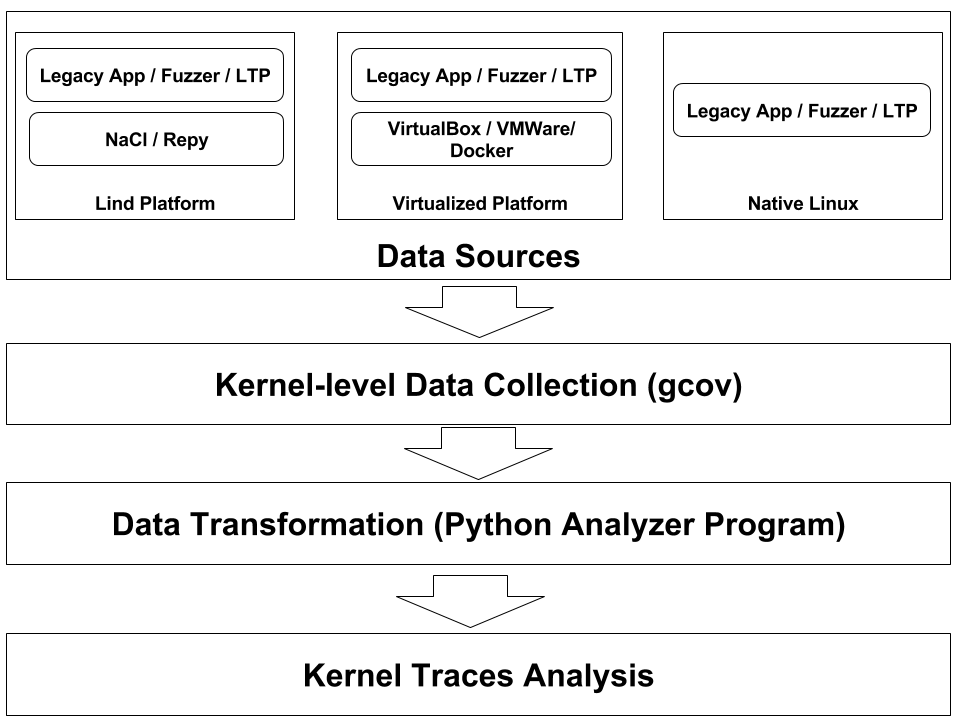
\includegraphics[width=1.0\columnwidth]{diagram/data_collection.png}
\caption{Various activities that were performed to capture and analyze the kernel
 traces generated by legacy applications, system fuzzers, LTP, and CVE bug
 reports. The traces are collected using \texttt{gcov} and a Python-based program that will transform the gcov data to 
 macrodata-level information of each travsersed path for final data analysis.}
 %\lois{transformed to what? And, how?

\label{fig:datacollection}
\end{figure}

We were able to assess the total reachable kernel paths through combining the kernel traces generated by Trinity and LTP. 
The results show that 38.5\% of the total reachable
kernel paths are commonly used. More importantly, only 2.5\% of the total studied bugs had traces in the common paths, 
while 50\% of the bugs were resided in the total reachable kernel paths which is an indication of residing less bugs in common paths compared to uncommon paths.
 
%\yanyan{I feel this is a bit early to make this conclusion.}
%\lois{does the slight wording change answer your concern, Yanyan?}

\subsubsection{Coverage Analysis of Common Paths}

The kernel trace coverage of the common paths and the total reachable paths
are shown in Figure \ref{fig:coverage}. The results show that the size of commonly-used kernel paths is small,
merely 12.4\% of the entire kernel code base. The common paths coverage is also significantly smaller than 
the total reachable paths coverage (about 1/3 of the entire kernel).

It may appear surprising that the total reachable paths coverage is low,
and accounts for only about one-third of the entire kernel. However,
this is consistent with kernel code coverage analysis
measurements conducted by other researchers \cite{LTP-Coverage}.
One reason that this occurs is that many paths
in the kernel cannot be accessed from the system call API. Another reason
is that
while obtaining the kernel coverage data, as most researchers did, we used
a system call fuzzing tool
and a Linux test suite to generate the kernel trace. These existing
tools do not reach every possible path in the kernel, due to
the fact that there are some limitations on the iteration number of issuing
the fuzzing calls. In addition, some kernel paths can only be reached by
certain combinations of different function calls with specific arguments.


\begin{figure}%[h]
\centering
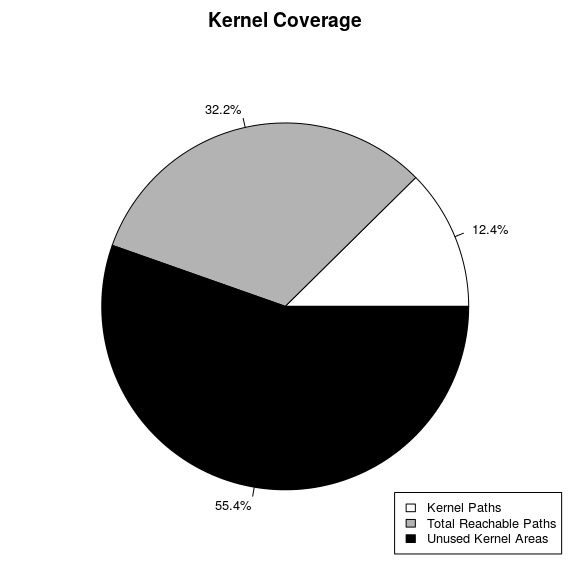
\includegraphics[width=1.0\columnwidth]{diagram/kernelcoverage.png}
\caption{Percentage of different kernel areas that were reached during
 LTP and Trinity system call fuzzing experiments.}
\label{fig:coverage}
\end{figure}


%Although the total reachable paths coverage is not 100\% of the entire
%kernel code base,
%it is still very large and contains many bugs.
%However, because the commonly used kernel path coverage is much smaller
%than
%the total reachable path coverage, this is a positive indication that these
%relatively small areas can be considered safe.

%\begin{table}
%\centering
%\scriptsize
%\caption {Kernel Coverage}
%\begin{tabular}{|l|c|}
%  \hline
%  \textbf{Kernel Paths} & \textbf{Kernel Coverage (percentage)} \\
%  \hline \hline
%  Common Paths & 12.4\% \\
%  \hline
%  Total Reachable Paths & 32.2\% \\
%  \hline
%\end{tabular}
%\label{table:kernel_coverage}
%\end{table}

The results from Figure \ref{fig:subset} and Figure \ref{fig:key_paths_trace}
show that the common paths are a subset of the
total reachable paths.
In Figure \ref{fig:subset} and Figure \ref{fig:key_paths_trace},
the ``OverlappedLines'' indicate the lines of code
in the kernel that appear both in the common paths and the total reachable
paths. While the ``UniqueLines'' show the lines of code that only appear in
the total reachable paths.

In Figure \ref{fig:subset}, the ``UniqueLines''
represent a large portion of the total reachable paths, more than 90K LOC.
Those lines of code are not executed by popular applications, which can be
potentially dangerous.

In Figure \ref{fig:key_paths_trace}, \texttt{fs}, \texttt{kernel/sched},
and \texttt{mm} refer to the total number of lines of code in that Linux kernel path.
Figure \ref{fig:key_paths_trace} shows that
substantial amount of code are found only inside the total reachable paths,
for some essential kernel paths like \texttt{fs} (6.5K LOC),
\texttt{kernel/sched} (3K LOC),
and \texttt{mm} (8K LOC).
A main reason for this outcome is that many lines of code in those kernel paths
are inside if conditions, and can only be reached by using special or
rare arguments and flags. Since the daily-used operations of
the popular applications do not require those kind of rare arguments
and flags, those ``UniqueLines'' only exist in the total reachable paths.

We closely examined the kernel trace derived from common paths
and the total reachable paths. We found that for each different path
in the kernel, the lines of code
in the common paths trace also appeared in the total reachable paths trace.
But there are many lines of code (more than 50\%)
in the total reachable paths trace that are not in the common paths. This
shows that the common paths trace and
the total reachable paths we obtained are as expected, because common paths in
the kernel should definitely be reachable.
One further finding is that the common paths account
for only 38.5\% of the total reachable paths.
This suggests that a large portion (61.5\%) of the kernel is not frequently
used by popular applications on a daily basis.

\begin{figure}
	\centering
	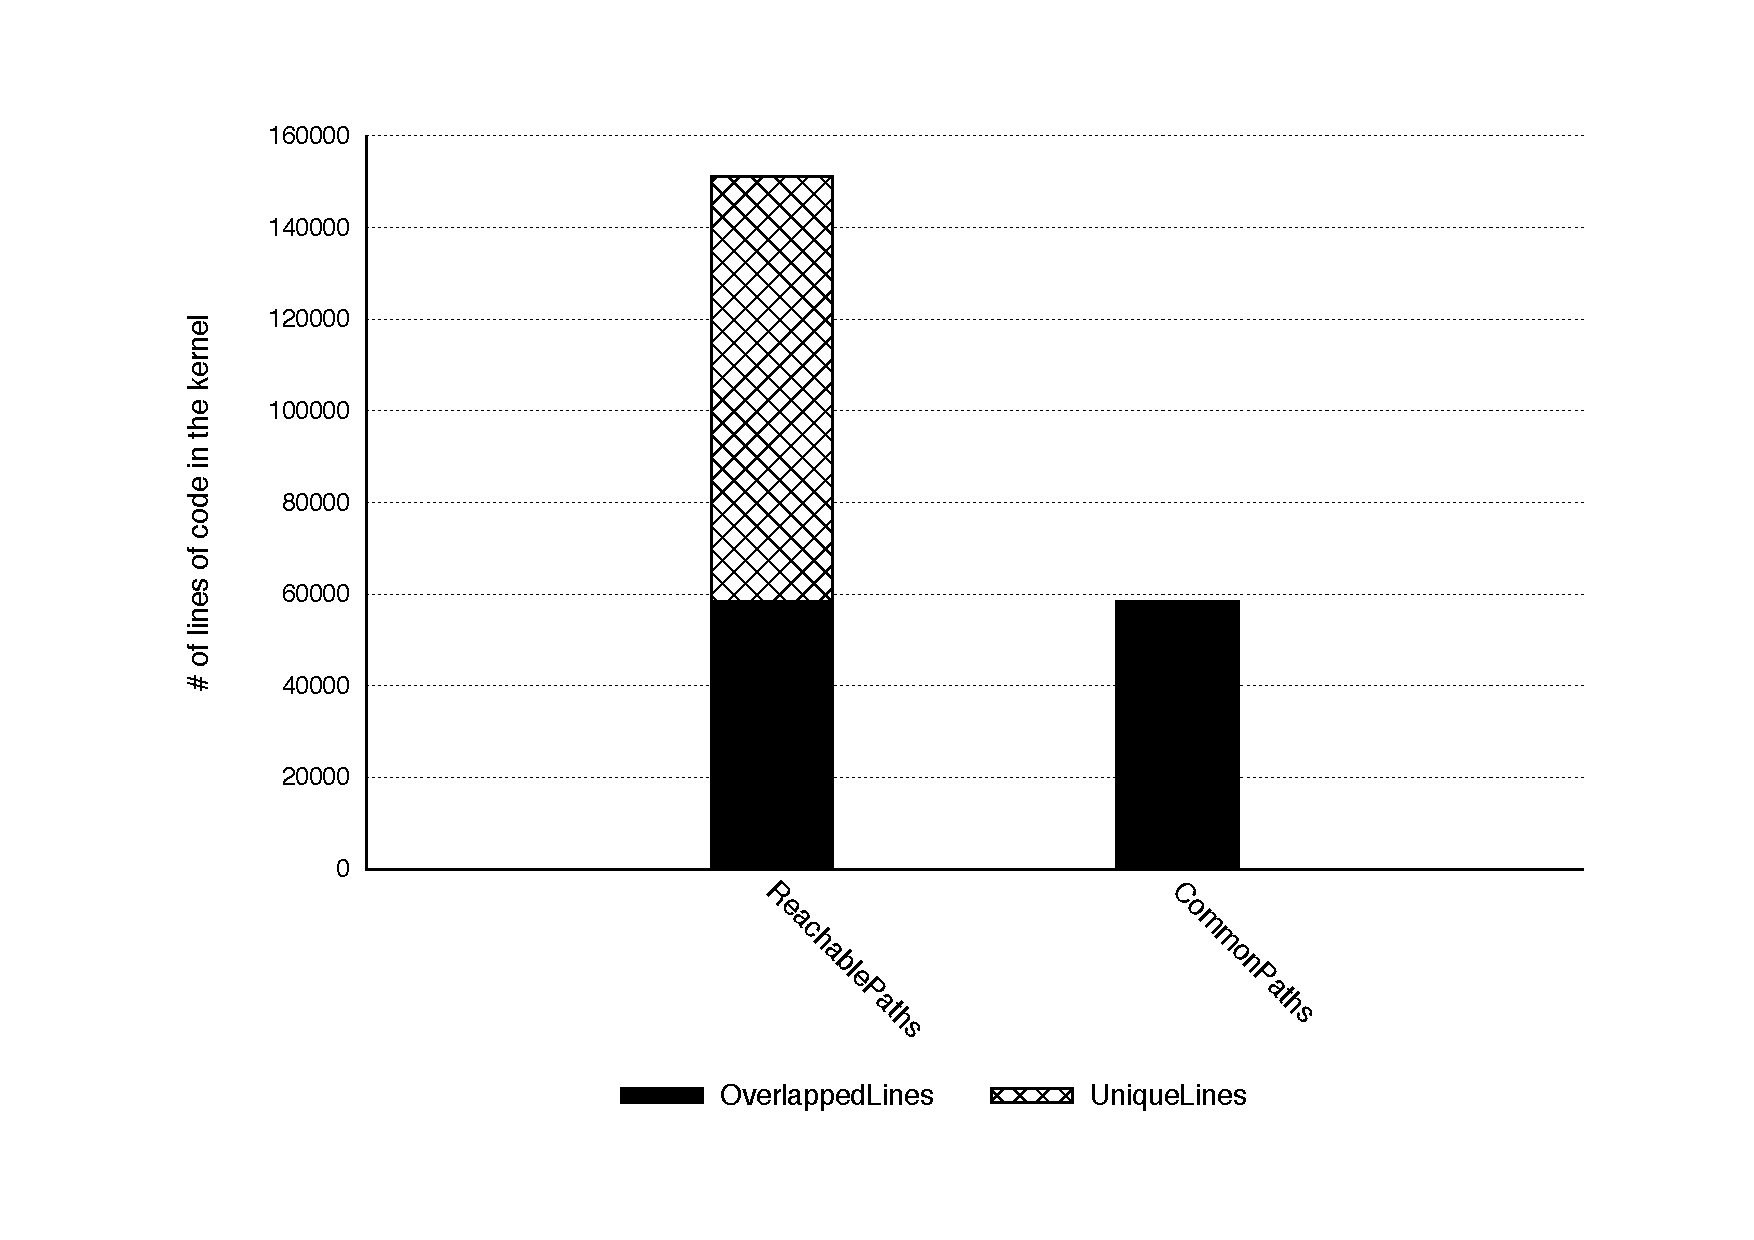
\includegraphics[width=1.0\columnwidth]{diagram/lind_oakland16_diagram_01.pdf}
	\caption{Kernel Trace Comparison: Common paths as a subset of reachable paths}
	\label{fig:subset}
	\end{figure}

	\begin{figure}
	\centering
	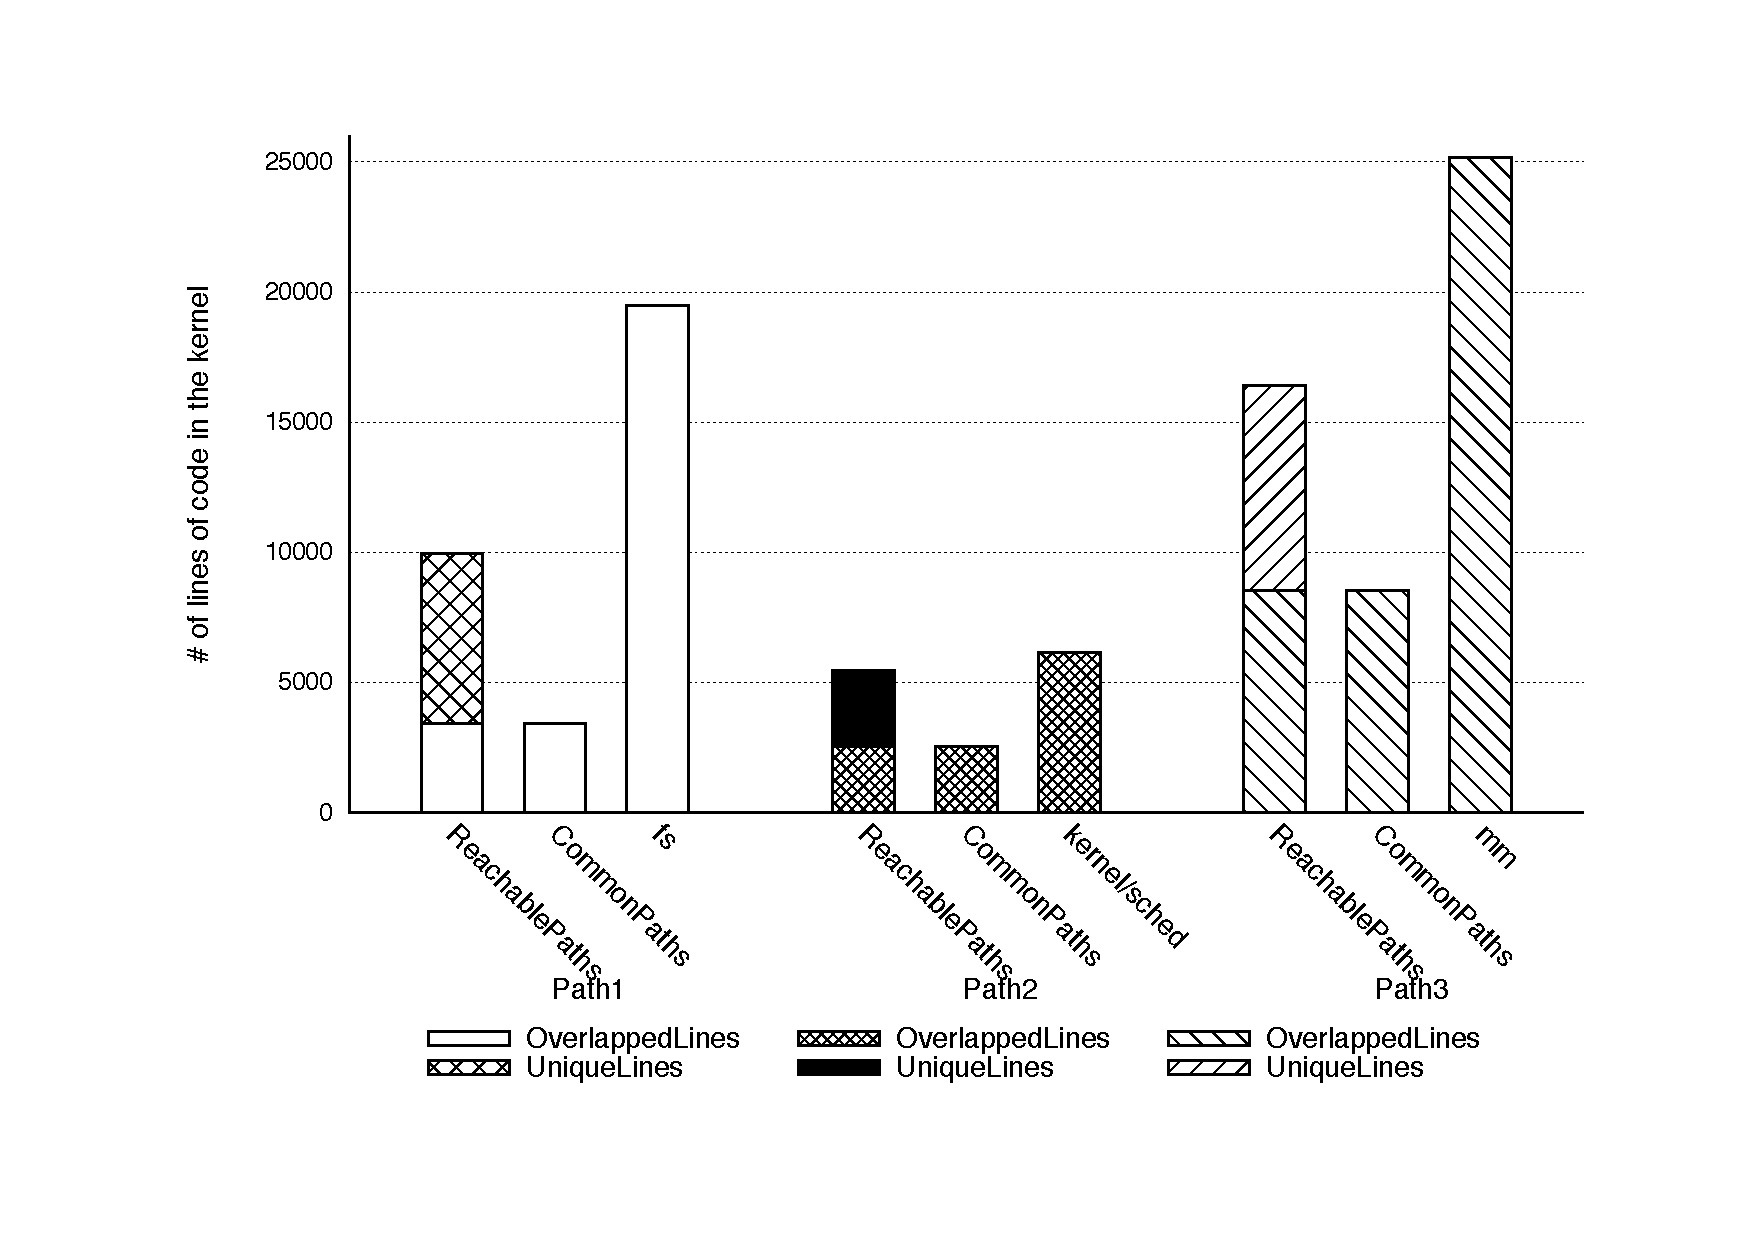
\includegraphics[width=1.0\columnwidth]{diagram/lind_oakland16_diagram_02.pdf}
	\caption{Kernel Trace in Key Paths}
	\label{fig:key_paths_trace}
\end{figure}

\subsubsection{Security Analysis of Kernel Paths\textendash Locating the
Risky Portions}

To verify our hypothesis, we next checked which portions of
the kernel contained kernel bugs. We examined 40 severe Linux kernel
sbugs that had been discovered by the research community in the last five
years (the first two columns in Table
\ref{table:vulnerabilities_commonly_used_kernel_paths}).
Those 40 bugs were chosen from the NVD bug database, according to
the vulnerability severity score assigned to them. We started with the ones
that have the highest severity score.
We used these kernel bugs to check if vulnerabilities existed in certain
kernel traces. This is done by comparing the kernel traces with the lines
of code we labeled for each bug, based on change of lines in the
kernel patch.

The results of our experiment are shown the last two columns in Table \ref{table:vulnerabilities_commonly_used_kernel_paths}.

\begin{table*}[!ht]
\scriptsize
\centering

\caption {Linux Kernel Bugs, and Vulnerabilities in Different Portions of
the Kernel
({\color{red}\ding{51}}: vulnerability in paths; \ding{55}: vulnerability
not in paths)}

\begin{tabular}{|l|l|c|c|}\hline
\multirow{2}{*}{\textbf{Vulnerability}} & \multirow{2}{*}{\textbf{Specific
Type}} & \multicolumn{2}{c|}{\bf Portion of the Kernel} \\
\cline{3-4}
&  & \textbf{Total Reachable Paths} &  \textbf{Common Paths} \\ \hline

 CVE-2014-9529 & concurrency, race condition & {\color{red}\ding{51}} &
\ding{55} \\
 CVE-2014-3631 & NULL pointer dereference & {\color{red}\ding{51}} &
\ding{55} \\
 CVE-2012-6657 & network socket variable mischeck & {\color{red}\ding{51}}
& \ding{55} \\
 CVE-2014-5207 & privilege escalation & \ding{55} & \ding{55} \\
 CVE-2014-5206 & privilege escalation & \ding{55} & \ding{55} \\
 CVE-2014-3153 & privilege escalation & \ding{55} & \ding{55} \\
 CVE-2014-2851 & privilege escalation & \ding{55} & \ding{55} \\
 CVE-2014-2706 & race condition, DoS & {\color{red}\ding{51}} & \ding{55}
\\
 CVE-2014-0100 & race condition, DoS & {\color{red}\ding{51}} & \ding{55}
\\
 CVE-2014-0049 & buffer overflow & \ding{55} & \ding{55} \\
 CVE-2012-6638 & DoS & {\color{red}\ding{51}} & \ding{55} \\
 CVE-2014-0038 & privilege escalation & \ding{55} & \ding{55} \\
 CVE-2013-6368 & privilege escalation & \ding{55} & \ding{55} \\
 CVE-2013-4587 & index error, privilege escalation & \ding{55} & \ding{55}
\\
 CVE-2013-4563 & size/boundary check, DoS & {\color{red}\ding{51}} &
\ding{55} \\
 CVE-2013-4348 & value validation error & \ding{55} & \ding{55} \\
 CVE-2013-4300 & privilege escalation & {\color{red}\ding{51}} & \ding{55}
\\
 CVE-2013-1943 & privilege escalation & \ding{55} & \ding{55} \\
 CVE-2013-2094 & privilege escalation & {\color{red}\ding{51}} & \ding{55}
\\
 CVE-2013-3301 & NULL pointer dereference, DoS & {\color{red}\ding{51}} &
\ding{55} \\
 CVE-2013-1858 & privilege escalation & {\color{red}\ding{51}} & \ding{55}
\\
 CVE-2013-1797 & use-after-free & {\color{red}\ding{51}} & \ding{55} \\
 CVE-2013-1763 & privilege escalation, index error & \ding{55} & \ding{55}
\\
 CVE-2013-0310 & NULL pointer dereference & \ding{55} & \ding{55} \\
 CVE-2012-2136 & heap-based buffer overflow & \ding{55} & \ding{55} \\
 CVE-2012-2100 & lack of sanity check  & \ding{55} & \ding{55} \\
 CVE-2012-0028 & privilege escalation & {\color{red}\ding{51}} & \ding{55}
\\
 CVE-2011-2517 & privilege escalation, buffer overflow &
{\color{red}\ding{51}} & \ding{55} \\
 CVE-2012-2123 & privilege escalation  & {\color{red}\ding{51}} & \ding{55}
\\
 CVE-2012-1146 & NULL pointer dereference  & \ding{55} & \ding{55} \\
 CVE-2012-0207 & divide-by-zero error and panic & \ding{55} & \ding{55} \\
 CVE-2011-2525 & NULL pointer dereference  & {\color{red}\ding{51}} &
\ding{55} \\
 CVE-2011-1076 & NULL pointer dereference  & {\color{red}\ding{51}} &
\ding{55} \\
 CVE-2011-2184 & NULL pointer dereference, none initialization & \ding{55}
& \ding{55} \\
 CVE-2010-2478 & integer overflow & {\color{red}\ding{51}} & \ding{55} \\
 CVE-2010-2960 & NULL pointer dereference  & \ding{55} & \ding{55} \\
 CVE-2010-2492 & privilege escalation, buffer overflow & \ding{55} &
\ding{55} \\
 CVE-2010-2240 & stack overflow & {\color{red}\ding{51}} &
{\color{red}\ding{51}}\\
 CVE-2010-1188 & use-after-free & \ding{55} & \ding{55} \\
 CVE-2010-0437 & NULL pointer dereference  & {\color{red}\ding{51}} &
\ding{55} \\ \hline
 \multicolumn{2}{|c|}{\bf Percentage contains bugs} & {\bf $50\%$} & {\bf
$2.5\%$} \\ \hline
\end{tabular}
\label{table:vulnerabilities_commonly_used_kernel_paths}
\end{table*}

The results of this analysis suggest that commonly used kernel paths contain only 2.5\% of all the bugs that we studied. 
Since the total reachable kernel paths contain 50\% of the bugs that were examined in this paper, we can conclude 
that commonly used kernel paths clearly contain fewer bugs than other portions of the kernel.

%We studied bugs from the large-scale NVD database which includes representative bugs for all categories, 
%and conducted experiments with ones with the highest vulnerability severity scores. This makes it a fair collection of available bugs sample 
%to ensure the sample was not biased and it would be a normal distribution of bugs in the Linux kernel. 
%\lois{Why does thismethod, which seems less than random, prove it is not biased?}


%Our hypothesis and findings provide insights and guidelines for new designs of secure systems, which will be discussed in the next section. 
%\cappos{Is this statistically significant?} 
%\yiwen{I added something to explain our bug sample dataset. More knowledge of statistics may be required. I will think about it more.}
\section{Motivation and Background}
\label{sec.motivation-and-background}

This section presents background information
relevant to the development of our design metric and the Lind prototype. We
start by exploring the function of the kernel and why protecting its
vulnerabilities is so difficult. We then present some assumptions about
the nature of an attack that could trigger those vulnerabilities.
%caused by an inability to identify which portions of the kernel are risky.

\subsection{Kernel Function and Vulnerabilities}

Running user applications relies on their ability to access
critical resources from the kernel, such as memory, I/O, or CPU.
The kernel provides interfaces to serve these requests
and essential functionality for all applications running in the system.
Thus all code, whether sandboxed or untrusted, will make calls
that are eventually processed by the kernel.

Unfortunately, OS kernels are vulnerable to adversarial attacks, which have
increased in frequency over time.
Over the past few years, exploitation of OS kernels has been wide-spread,
despite substantial efforts by researchers and practitioners.
In 2014, 215 vulnerabilities in all types of kernels were reported~\cite{NVD},
of which 125 were in the Linux kernel alone.
With the constant addition of new features~\cite{Metrics-13}, the kernel's
attack surface keeps increasing For example, the Linux kernel grew from 6.6 MLOC
in v2.6.11 (March 2005) to 16.9 MLOC in v3.10 (June 2013)~\cite{Linux-13}.

\cappos{Likely cut this.  I think it is excessive.}

Such a huge kernel codebase has lead to excessive exploitation, where it has
been plagued by a number of common software flaws.
These flaws have raised serious security concerns and caused severe damage
to systems.\lois{Are these sentences needed? Is this what Justin thought was
excessive? If so, I agree.} The common vulnerability and exposure (CVE) database
reports indicate stack and heap buffer overflow vulnerabilities
have been used to launch denial of service attacks through crashing the systems
 (CVE-2013-2892).
%~\cite{CVE-2013-2892},
Other vulnerabilities such as the execution of arbitrary code (CVE-2009-3234)
%~\cite{CVE-2009-3234},
or to allow local users to gain privileges via a crafted
application (CVE-2013-1828) are also among the reports.
%~\cite{CVE-2013-1828}.
Memory disclosure vulnerabilities (CVE-2009-3002) have been also exploited to allow local users
to read
the contents of some kernel memory locations
%~\cite{CVE-2009-3002}
, or to obtain potentially sensitive information from kernel stack memory (CVE-2010-4073).
%~\cite{CVE-2010-4073}.
Attackers have also used use-after-free vulnerability to gain kernel
privileges, i.e. CVE-2013-4343.
%~\cite{CVE-2013-4343}.\lois{If this is what Justin thought was excessive, I
would still agree. It is too much of a "laundry list" of random examples, with no
specifics.}

%The number of kernel vulnerabilities and their potential for exploitation,
%plus the fact that user applications rely on the kernel to execute
%programs,
%present a compelling motive for designing securer systems that can run
%applications with a better degree of safety. \yanyan{this paragraph does
%not say anything new.}

\subsection{Threat Assumptions}

The primary goal of a secure system is to restrict a program to a subset
of privileges. Most systems mediate this access to the underlying operating
system through a set of functions.
Threats occur when applications obtain access to privileges that were not
intentionally granted by the system, and thus the system loses the intended
protection~\cite{Repy-10}.
To apply the proposed security metric to a developing lois{developing?} system,
we make the following assumptions:

\begin{enumerate}
\item The OS kernel contains at least one bug that is known to an adversarial attacker.

\item The attacker has the ability to execute code inside
of a virtualized system, such as an operating system VM or library OS.
This access may be obtained by writing a malicious application
that the user executes, or by exploiting a flaw that exists in a user's
application.

\item Unintentional bugs may exist in any complex code. This
includes any security systems placed between the kernel and the user
applications.

\item Some form of computational containment can feasibly be implemented.
This means that an isolated program cannot simply
make arbitrary system calls and access the kernel directly. This containment could
be provided through software-fault isolation~\cite{SFI:93}, programming
language techniques\cappos{cites}, or by running isolated code in a
distinct region of virtual memory\cappos{cites}.

\item It is possibile to build functionality that possesses few
vulnerabilities as long as the code-base is kept to a minimum.

\cappos{How do I explain
the sandbox TCB???  How is this different from a hypervisor?}

\end{enumerate}
\section{A New Design for Building Secure Virtualization Systems}
\label{sec.design}

This section discusses how to use the observation
 that ``commonly used kernel paths'' contain fewer bugs 
(\S{\ref{sec.metric}}) to build securer virtualization systems.
The key idea of our design is that all code \emph{including the complex part
of the operating system API} should have a very small TCB that accesses only 
commonly used kernel paths. 
Any complex or possibly risky system functions 
are reimplemented by our own code within a sandbox. This makes any bugs or failures within the implementation of those complex system functions 
to be contained by the sandbox. As result untrusted code will not have the possibility to reach 
and trigger sensitive and risky portions of the kernel. 


\begin{figure}%[h]
\centering
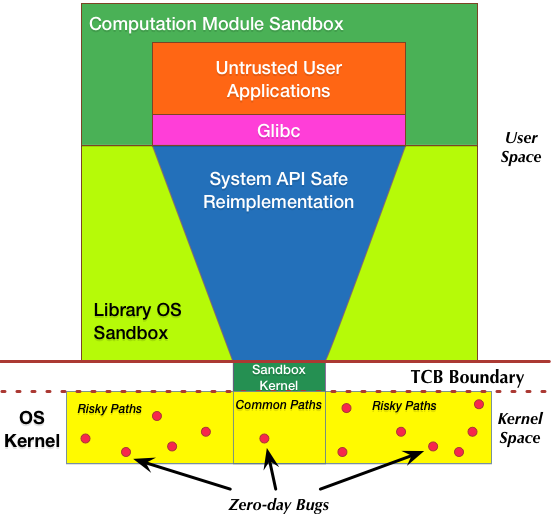
\includegraphics[width=1.0\columnwidth]{diagram/lind_secure_design_new.png}
\caption{``Safe-Reimplementation'' design to ensure predictable execution of untrusted user codes despite existing potential zero-day bugs within the OS kernel.} 
\label{fig:design}
\end{figure}

\subsection{Architecture}

To execute untrusted applications in a safe manner that will not trigger bugs 
in the underlying OS kernel, %and cause damage to other parts of the system, 
we must build a sandbox system that can provide isolation and 
containment for any improper operations in the programs. 
One approach to building such a system is to place it entirely in the user space, 
and to only have a small sandbox kernel with restricted access to the OS kernel (Figure \ref{fig:design}). 
This approach has advantages over other approaches that require modifications to 
the OS kernel, as it avoids the risk of threat escalation. If modified modules 
are inside the OS kernel, they have kernel privileges that could allow attacks on the underlying OS, 
as well as applications run on top of it. 

There are two main components in our design of a secure virtualization system, as shown in Figure \ref{fig:design}. 
The first is a computation module, which performs functions like type checking, object creation, 
and garbage collection. The second is a system API that serves requests to access the OS kernel. 
Those two components should work together to complete the requirements of running user code. 
To run this code in our sandbox system, we first invoke the computation module to perform its operations. 
Whenever there are system call requests, 
the computation module will direct those requests to our system API. 
The system API will respond to the system call requests and return results to the user code if the requests are granted. 

\subsubsection{The Computation Module}

Our secure system should be able to support and run legacy applications, 
and execute binary code compiled from unmodified source code on popular hardware architecture, 
like x86 architecture. Providing an execution environment that can run unmodified source code is 
the main responsibility of the computation module. The key security issue of executing system calls 
without triggering OS kernel bugs is left to the system API module.

\subsubsection{The System API Module}

The system API module is the core of our sandbox system. It is comprised of two parts, 
a sandbox kernel that provides access to basic but critical system calls, and a system 
API safe reimplementation that implements more complex calls. 

The sandbox kernel forms the only addition to the TCB of our system.  We 
make this system extremely small and simple so that it is easy to verify its 
security.  The purpose of the sandbox code is simply to provide an API that performs
a few critical system calls with the most basic parameters.  For example,
programs will need some mechanism to write data to the file system
and communicate with the network.  The kernel's goal is to provide the ability
to do so, while utilizing the most simplistic calls possible with the most
basic arguments.  For example, the file system API need only provide a way
to write data to storage.  It need not provide a directory abstraction, the
concept of file permissions, links, or even the concept of multiple files.
It merely needs to provide a mechanism to write out data that can be later
read in.  

%It should have a set of capabilities that enable the construction of essential and more complicated functions. 
%For example, the sandbox kernel capabilities should include basic functions for network, 
%file system I/O, lock, thread, and namespace. It also needs to have access to the OS kernel through system calls. 
%In developing our design, we leveraged our verified hypothesis that commonly used kernel paths contain fewer bugs. 
%Thus, the system calls we allow in our sandbox kernel are common calls, like file open, read, write, and close. 
%Furthermore, the set of arguments used for each call is also highly restricted. 

The system API safe reimplementation is a set of more complicated system calls 
that are constructed from our sandbox kernel. It should be able to reconstruct 
complex system functions, like those complex calls in the file system API. 
We reimplemented those system calls because we did not want user code 
to have direct access to the underlying OS kernel. 
Therefore, our reimplementation layer serves as a mediator between the user code 
and the OS kernel. In our design, the reimplementation is safe 
because the reconstruction of system calls is isolated in a sandbox. 
This can be done by choosing a memory-safe programming language to write code for the reimplementation. 
With this design, even if there are bugs in the function reimplementation, 
they cannot escape from the sandbox and will not reach the underlying OS kernel. 

Here is an example of how this reimplementation would work with the symbolic link function. 
If there is a bug in this function, our safe reimplementation will not rely on the kernel code paths for symbolic links. 
Instead, our sandbox system will implement the incorrect behavior, so the program will not be forced to quit, but will do so in the sandbox. 
\yanyan{why implement the buggy behavior?}  
Since the reimplementation code does not have privileged access to the system as the OS kernel does, 
this will not result in a security issue. The usual outcome of a bug in this case is simply that the application will fail.

With the computation module and the system API module, unmodified user code is able to run on top of our designed system. 
It is important to note that our design does not rely on any specific technique or tool. 
To implement the computation module and the system API module in our design, 
it is possible to choose from several different techniques that fit well with the users' specific needs or requirements.

This general system design was implemented as a prototype called Lind. 
In the next section, we provide a detailed description of Lind.

\subsection{Discussion: Our Design Choice}

In reviewing our design, some fundamental questions could be raised about the dual sandbox design. 
Why is one not enough? And, if two is good, why not use three or more? 
The answer to the first question is that the kernel interface is extremely rich and hard to protect. 
In order to have minimal impact on the kernel, as well as provide sufficient API for legacy applications, 
we need to have one sandbox focuses on protecting the kernel and providing POSIX API, 
while a second sandbox focuses on efficiently executing applications. 
So our approach includes two sandboxes, one as the computation module, 
and the other one as system API module. As to the second question, 
which could be rephrased as ``why not sandbox Repy TCB and get more security?,'' 
the lowest level sandbox eventually must have some fundamental, 
even if  limited access to system resources, such as memory, and storage, threads. 
So even if we were to sandbox Repy TCB and have additional sandboxes, 
the one at the bottom level will still access the OS kernel in a similar way. 
Thus, having multiple sandboxes does not provide any extra security benefits. 

\section{Implementation of the Lind Prototype}
\label{sec.implementation}

Based on the design introduced in Section \ref{sec.design},
we implemented a secure sandbox system, Lind,
for running untrusted user programs on vulnerable OS kernels.
Lind adapts two basic technologies as its building blocks\textendash
Google's Native Client (NaCl), and Seattle's Repy.

As described in Figure \ref{fig:design}, our design has
two main components\textendash a computation module that isolates the
application and a library OS module that isolates the complex
portions of POSIX, a standard OS interface Lind provides
We choose Google's Native Client (NaCl) ~\cite{NaCl-09} as the computation
module because NaCl is a widely used environment for efficient execution of legacy code in the
form of x86 and ARM binaries. 
Seattle's Repy is used as our library OS module (Figure \ref{fig:architecture}), since it is a restricted subset of Python, 
that works as a sandbox to provide a safer environment to run untrusted code.

\begin{figure}%[h]
\centering
	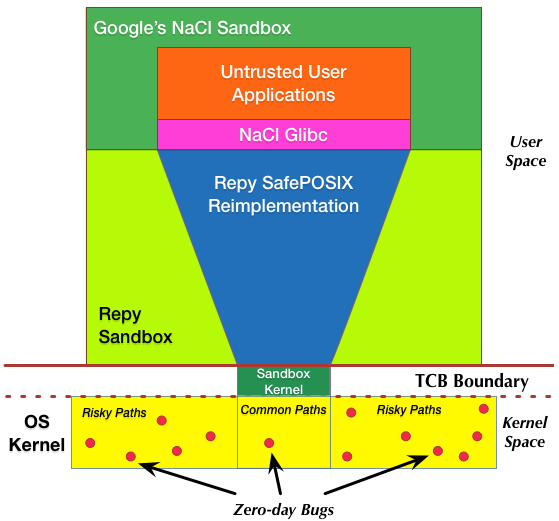
\includegraphics[width=1.0\columnwidth]{diagram/lind_architecture_new.png}
	\caption{Architecture of Lind including various components such as NaCl, NaCl glibc, and Repy Sandbox.
	User level application issues system calls that are dispatched through the Repy OS connector that bridges the Lind system to the OS Kernel.}
\label{fig:architecture}
\end{figure}

\subsection{The Computation Module of Lind: Google's Native Client}

We utilize NaCl in our design to isolate the computation of the user application 
from the kernel.
NaCl allows Lind to work on most types of legacy code.
It compiles the programs to produce a binary with software fault isolation.
This prevents the majority of the application from performing system calls
or executing arbitrary instructions.

To perform a system call, the application will call into a small privileged
part of the NaCl TCB that forwards system calls, usually to the OS or to Chrome for
processing. To build Lind, we changed the NaCl TCP to
instead forward these calls to our library OS module that we call SafePOSIX implementation
for processing. The NaCl
glibc module contains stubs that reject operations
that Chrome would not handle.  We added functionality to NaCl's glibc so that
those calls could be forwarded into SafePOSIX for processing.

%NaCl can perform the functions required by the computation module well, and it is easy to
%connect with our system API module because NaCl uses glibc to perform system calls.
%Modification to NaCl's glibc would allow us to redirect those system call requests to our own system API module.
%
%NaCl is a sandbox used to execute untrusted x86 native code.
%It aims to give applications the computational performance of native applications without compromising safety.
%NaCl uses software fault isolation and a secure runtime to direct system interaction and
%side effects through interfaces managed by the program. It provides operating system portability
%for binary code while supporting performance-oriented features, such as thread support,
%instruction set extensions, such as SSE, and use of compiler intrinsics and a hand-coded assembler.
%It also allows the efficient execution of legacy code in the form of x86 and ARM binaries
%that are built with a lightly modified compiler tool chain.

\subsection{The Library OS Module of Lind: Seattle's Repy}

To build an API to access the safe parts of the underlying kernel, we need
two things.  First, we need a restricted sandbox that isolates computation
and only allows access to commonly used kernel paths.  We used
Seattle's Repy~\cite{Repy-10} sandbox to perform this task.
Second, we need to build a POSIX implementation to run within that sandbox.

%pplications. For Lind, we used Repy to build our system API module.
%To be more specific, our system API module has a very small sandbox kernel
%as TCB,  written with Python. On top of the sandbox kernel,
%we use Repy code to safely reimplement complex system functions.

\subsubsection{The Repy Sandbox Kernel}

As discussed earlier in Section \ref{sec.design}, the sandbox kernel needs to be secure and bug-free.
Because it is the TCB of the system, any bugs within it could cause fatal problems,
and allow attackers to access the OS kernel and gain kernel privilege.
We used Seattle's Repy system API module due to its tiny sandbox kernel
(comprised of only around 8,000 LOC)lois{is LOC always recognized ore should it be defined the
first time it appears?}. Using Repy also fit our key design principle that
our proposed system should only access the safe portions of the OS kernel.
The Repy sandbox kernel, has 33 basic API functions, including 13 network functions,
6 file functions, 6 threading functions,
and 8 miscellaneous functions
 (Table \ref{table:RepyKernel}) \cite{Repy-10}, \cite{RepyKernel}. Most of those functions are simple and
regularly used system calls that access the commonly used kernel paths.


\begin{table}
\centering
\caption {Repy sandbox kernel capabilities that supports NaCl functions, such as networking, file I/O operations and threading.}

  \begin{tabular}{ | p{2.5cm} | p{4.5cm} |}
  \hline
  \textbf{Repy Function} & \textbf{Available System Calls}  \\ \hline

Networking & \emph{gethostbyname, openconnection, getmyip, socket.send, socket.receive, socket.close,
listenforconnection, tcpserversocket.getconnection, tcpserversocket.close, sendmessage, listenformessage,
udpserversocket.getmessage, and udpserversocket.close.} \\ \hline

I/O Operations & \emph{openfile, file.close, file.readat, file.writeat, listfiles, and removefile.} \\ \hline

Threading & \emph{createlock, sleep, lock.acquire, lock.release, createthread, and getthreadname.} \\ \hline

Miscellaneous Functions & \emph{getruntime, randombytes, log, exitall, createvirtualnamespace,
virtualnamespace.evaluate, getresources, and getlasterror.}  \\ \hline
    \end{tabular}
    \label{table:RepyKernel}
\end{table}

%\begin{table}
%\centering
%\scriptsize
%\caption {System Functions in the Repy Sandbox Kernel.  \cappos{Need to
%clearly explain the takeaway.}}
%\begin{tabular}{|l|}
%  \hline
% \textbf{Network Functions} \\
%  \hline
%  gethostbyname(name) \\
%  \hline
%  getmyip() \\
%  \hline
%  openconnection(destip, destport, localip, localport, timeout) \\
%  \hline
%  socket.close() \\
%  \hline
%  socket.recv(numbytes) \\
%  \hline
%  socket.send(message) \\
%  \hline
%  listenforconnection(localip, localport) \\
%  \hline
%  tcpserversocket.getconnection() \\
%  \hline
%  tcpserversocket.close()\\
%  \hline
%  sendmessage(destip, destport, message, localip, localport) \\
%  \hline
%  listenformessage(localip, localport) \\
%  \hline
%  udpserversocket.getmessage() \\
%  \hline
%  udpserversocket.close() \\
%  \hline \hline
%  \textbf{File Functions} \\
%  \hline
%  openfile(filename, create) \\
%  \hline
%  file.close() \\
%  \hline
%  file.readat(sizelimit, offset) \\
%  \hline
% file.writeat(data, offset) \\
%  \hline
%  listfiles() \\
%  \hline
%  removefile(filename) \\
%  \hline \hline
%  \textbf{Threading Functions} \\
%  \hline
%  createlock() \\
%  \hline
%  lock.acquire(blocking) \\
%  \hline
%  lock.release() \\
%  \hline
%  createthread(function) \\
 % \hline
 % sleep(seconds) \\
  %\hline
  %getthreadname() \\
  %\hline \hline
  %\textbf{Miscellaneous Functions} \\
  %\hline
 % getruntime() \\
  %\hline
 % randombytes() \\
  %\hline
  %log(*args) \\
  %\hline
  %exitall() \\
  %\hline
  %createvirtualnamespace(code, name) \\
  %\hline
  %virtualnamespace.evaluate(context) \\
  %\hline
  %getresources() \\
  %\hline
  %getlasterror() \\
  %\hline
%\end{tabular}
%\label{table:RepyKernel}
%\end{table}

A natural concern with any sandbox design is that bugs are simply pushed into
another part of the trusted code base.  As it is the only piece of code added
to the system call paths of the TCB, the Repy sandbox kernel's security is of
paramount concern.

The sandbox kernel consists of only XXXX lines of code \cappos{continue...}.
The code is written to provide straightforward access to the minimal set
of the system call API needed to build general computational functionality.
The code is written using style guidelines designed to ease security auditing
 of the code~\cite{style}.

The sandbox kernel code has been
audited by a professional penetration tester.  Since 2010, there has also been
a bug bounty program for security flaws in the sandbox.
The code is deployed in daily use across thousands of devices,
including on the Seattle testbed \cite{seattle}, and has been examined by
hundreds of parties.  Developers have reported
XXX issues for problems in other parts of the systems. However, to date
no security flaws have been found in the sandbox kernel.
This does not provide any strong guarantees that bugs could not exist, and if
they do, the security of the system could be compromised.
However, having a small, easily auditable piece of code helps to reduce the
risk of this occurrence.

\subsubsection{The SafePOSIX Reimplementation}

The key responsibility of our system API module is to serve system call requests from user code.
In the Lind system, those system call requests are issued from the user code,
received by the computation module NaCl, and then redirected to our system API module.
The API module includes a POSIX API to serve those requests.

A POSIX API is a set of standard operating system interfaces that provide operating system functions
to the user code. However, the POSIX API is large and complex enough that its is
very hard to ensure that its implementation is secure and bug-free.\lois{Make sure this sentence
is correct. It was actually saying the opposite when I saw it yesterday. In discussion with
Yiwen I added the negative. But doublecheck.}

Our choice to use Repy helped us solve this architectural security problem.
Since Repy is a programming language sandbox, it can provide the ideal isolation
we needed when constructing our POSIX API. In Lind,
complex system functions are reimplemented using Repy code,
based on the ``safe-reimplement'' principle from our design in \S{\ref{sec.design}}.

\subsection{Operations}

Lind combines the NaCl and Repy components to provide native computation and
safe access to the system. Untrusted programs are run in NaCl,
but access to all system resources is diverted to a Repy program.
This program is responsible for accessing the system on behalf of the Lind library
 OS. A NaCl sandbox is built on top of the Repy sandbox.

To service a system call in NaCl, a server routine marshals its arguments into a text string,
and sends the call and the arguments to Repy sandbox.
The library OS then executes the appropriate system call, marshals the result and
returns it back to NaCl. The result is eventually returned as the appropriate native type to the calling program.

Lind is designed to minimize the need to modify either sandbox. This is possible
because the TCB of both were extremely small, and because the Lind code is run
in both\lois{Another odd sentence Yiwen and I discussed. I thought I knew how to
fix it, but it still does not make sense. I would delete it.}

The only complex part of Lind is the library OS, which runs in Repy.
However, because Python is a very powerful language that provides rich functions,
it significantly simplified the construction of Lind. \lois{I'm still not sure
how Python simplified construction}. Even though Python is considered ``slow'' by some,
the internals of an application in Lind are run in NaCl, a very high performance
environment. \lois{sentence above must be deleted or rephrased unless we can produce
evidence that Python is considered "slow."}
This balances the performance of the system, with the ease of implementation and maintenance
of the library OS component of Lind.

The novel idea behind the architecture and design for sandboxing using Lind
ensures the programs are portable.\lois{the "novel idea" is never spotlighted}
Programs running inside Lind are written to work against \lois{I don't think "against"
is the right word here} a standard POSIX glibc interface,
and, since the Lind runtime is strictly user-level, it can work on many different platforms
including Linux, Mac OS X and Windows.

The lightweight and minimized overhead is another feature of Lind. Because the sandbox only
 incurs overhead when there is a system call, overall overhead for Lind is low.
 Yet, it does not sacrifice performance for cost.
Lind uses a native interface for execution,
allowing CPU-and-memory-intensive applications to run at speeds that are equivalent
 to NaCl and near native speed.


In Sectioin \ref{sec.evaluation}}, we report how the dual sandboxes and other elements
of Lind performed in head-to-head evaluation against other virtualization systems.
\section{Evaluation}
\label{sec.evaluation}

In order to evaluate Lind's effectiveness in providing kernel protection, we
conducted a series of experiments designed to answer four fundamental questions:

\begin{itemize}
\item How does the security of Lind compare to other virtualized environments?
(\S{\ref{Linux-Kernel-Bug-Test-and-Evaluation}})

\item How much of the underlying kernel is reachable in different
virtualization systems?
(\S{\ref{Reachable-Kernel-Trace-Analysis-for-Different-Virtualization-Systems}})

\item If the SafePOSIX implementation has bugs, how much more of the kernel would be
reachable?
(\S{\ref{Reachable-Kernel-Trace-Analysis-for-Repy-Sandbox}})

\item If the Repy sandbox kernel has bugs, how much of a threat does this pose?
(\S{\ref{Sandbox-Kernel-Bugs}})

\item If implemented, what is the expected overhead for Lind?
(\S{\ref{Performance-Evaluation}})
\end{itemize}

This section describes both the set-up of our experiment, and argues
how the results support the merits of our secure design and its Lind prototype.

\subsection{Evaluation Methodology}

Our evaluation strategy was to directly compare the performance of Lind
against
four other existing virtualization systems\textendash VirtualBox, VMWare
Workstation,
Docker, and Graphene. We also compared it against Native Linux and used
those results as a baseline for evaluation. Because Native Linux is the
original OS,
without virtualization and additional protection, this data helps to
clarify the security benefits of Lind,
as well as whatever performance overhead costs the system may incur.

\textbf{Experimental setup.}
We conducted our experiments under Linux kernel 3.14.1, using the following
protocols:

\begin{itemize}
\item We identified and examined a list of  69 historical bugs that have
specifically
targeted Linux kernel 3.14.1 \cite{CVE-Datasource}. By analyzing
security kernel patches for those bugs,
we identified the lines of code in the kernel that correspond to each
one.

\item In order to test if a bug can be triggered, we created or located C
code that can exploit each of the kernel bugs \cite{Exploit-Database}.
We were able to trigger and obtain results for
35 out of the 69 bugs in our experiments. We decided to focus our study on these
35 bugs and leave the other, more complex bugs, to future work and analysis
because we were either unable to find code that would trigger them at the moment,
or we could not clearly determine if triggering had occurred. \lois{I revised the
the previous sentence because it read a bit awkward, but it is still somewhat
clumsy. I'll try again in the next round of edits.}

\item We compiled and ran the exploit C code under each virtualization
system to
obtain their kernel traces, and then used our kernel trace safety metric to
determine
if a specific bug was triggered.

\item Lastly, to analyze the reachable kernel paths for each of the
virtualization systems,
we conducted system call fuzzing (similar to what we did in \S{\ref{sec.metric}}) to obtain
the kernel trace in each system.
We repeated the system call fuzzing within Repy as well to obtain its
kernel trace.
\end{itemize}

\subsection{Analysis of Study Results}

Guided by the study questions listed above, our tests were conducted and results
primarily goal from a security perspective.
(\S{\ref{Linux-Kernel-Bug-Test-and-Evaluation}} --
%\S{\ref{Reachable-Kernel-Trace-Analysis-for-Different-Virtualization-Systems}},
\S{\ref{Reachable-Kernel-Trace-Analysis-for-Repy-Sandbox}}).
However, to get some idea of its potential efficacy
in real-world settings, we also measured and evaluated the performance
overhead of Lind.
(\S{\ref{Performance-Evaluation}})

\subsubsection{Linux Kernel Bug Test and Evaluation}
\label{Linux-Kernel-Bug-Test-and-Evaluation}

We attempted to trigger 35 identified Linux kernel bugs by running programs in
Native Linux, VirtualBox, VMWare Workstation, Docker, Graphene,
and Lind, to evaluate if any of them can be triggered.\lois{Any particular
reason for choosing these bugs programs?} The kernel bugs
examined are capable of causing serious security problems. For example,
the CVE-2014-8989 bug allows local users to bypass intended file
permissions by leveraging a POSIX ACL.\lois{consequences of this?}
When running applications, the potential risk of triggering some of these
kernel bugs here,
and possibly many more bugs outside our list, is a severe problem that
users should be concerned about.\lois{Is the previous sentence needed?}

\begin{table*}%[!ht]
\scriptsize
\centering
\caption {Linux Kernel Bugs, and Vulnerabilities in Different
Virtualization Systems
({\color{red}\ding{51}}: vulnerability triggered; \ding{55}: vulnerability
not triggered).\cappos{It may be useful to add NaCl.  I suppose one could
argue that NaCl is really what is providing protection or that NaCl is good
enough.}}
\begin{tabular}{|l|c|c|c|c|c|c|}\hline
\textbf{Vulnerability}    &  \textbf{Native Linux}  &  \textbf{VirtualBox}
&  \textbf{VMWare Workstation}
 & \textbf{Docker} & \textbf{Graphene} & \textbf{Lind} \\
\hline
 CVE-2015-5706 & {\color{red}\ding{51}} & {\color{red}\ding{51}} &
{\color{red}\ding{51}} & {\color{red}\ding{51}} & {\color{red}\ding{51}} &
\ding{55}  \\
 CVE-2015-0239 & {\color{red}\ding{51}} & {\color{red}\ding{51}} &
{\color{red}\ding{51}} & \ding{55} & \ding{55}  & \ding{55}  \\
 CVE-2014-9584 & {\color{red}\ding{51}} & \ding{55}  & \ding{55}  &
\ding{55} & \ding{55}  & \ding{55}  \\
 CVE-2014-9529 & {\color{red}\ding{51}} & {\color{red}\ding{51}}  &
\ding{55}  & \ding{55} & \ding{55}  & \ding{55}  \\
 CVE-2014-9322 & {\color{red}\ding{51}} & {\color{red}\ding{51}}  &
\ding{55}  & {\color{red}\ding{51}} & {\color{red}\ding{51}}  & \ding{55}
\\
 CVE-2014-9090 & {\color{red}\ding{51}} & \ding{55}  & \ding{55}  &
\ding{55} & \ding{55}  & \ding{55}  \\
 CVE-2014-8989 & {\color{red}\ding{51}} & {\color{red}\ding{51}} &
{\color{red}\ding{51}} & {\color{red}\ding{51}} & {\color{red}\ding{51}} &
\ding{55}  \\
 CVE-2014-8559 & {\color{red}\ding{51}} & \ding{55}  & \ding{55}  &
\ding{55} & \ding{55}  & \ding{55}  \\
 CVE-2014-8369 & {\color{red}\ding{51}} & \ding{55}  & \ding{55}  &
\ding{55} & \ding{55}  & \ding{55}  \\
 CVE-2014-8160 & {\color{red}\ding{51}} & {\color{red}\ding{51}} &
{\color{red}\ding{51}} & \ding{55} & \ding{55}  & \ding{55}  \\
 CVE-2014-8134 & {\color{red}\ding{51}} & {\color{red}\ding{51}} &
{\color{red}\ding{51}} & \ding{55} & {\color{red}\ding{51}}  & \ding{55}
\\
 CVE-2014-8133 & {\color{red}\ding{51}} & {\color{red}\ding{51}}  &
\ding{55}  & \ding{55} & \ding{55}  & \ding{55}  \\
 CVE-2014-8086 & {\color{red}\ding{51}} & {\color{red}\ding{51}} &
{\color{red}\ding{51}} & {\color{red}\ding{51}} & \ding{55} & \ding{55}  \\
 CVE-2014-7975 & {\color{red}\ding{51}} & \ding{55}  & \ding{55}  &
\ding{55} & \ding{55}  & \ding{55}  \\
 CVE-2014-7970 & {\color{red}\ding{51}} & \ding{55}  & \ding{55}  &
\ding{55} & \ding{55}  & \ding{55}  \\
 CVE-2014-7842 & {\color{red}\ding{51}} & \ding{55}  & \ding{55}  &
\ding{55} & \ding{55}  & \ding{55}  \\
 CVE-2014-7826 & {\color{red}\ding{51}} & {\color{red}\ding{51}} &
{\color{red}\ding{51}} & \ding{55} & {\color{red}\ding{51}}  & \ding{55}
\\
 CVE-2014-7825 & {\color{red}\ding{51}} & {\color{red}\ding{51}} &
{\color{red}\ding{51}} & \ding{55} & {\color{red}\ding{51}}  & \ding{55}
\\
 CVE-2014-7283 & {\color{red}\ding{51}} & \ding{55}  & \ding{55}  &
\ding{55} & \ding{55}  & \ding{55}  \\
 CVE-2014-5207 & {\color{red}\ding{51}} & \ding{55}  & \ding{55}  &
\ding{55} & \ding{55}  & \ding{55}  \\
 CVE-2014-5206 & {\color{red}\ding{51}} & \ding{55}  &
{\color{red}\ding{51}}  & {\color{red}\ding{51}}& \ding{55}  & \ding{55}
\\
 CVE-2014-5045 & {\color{red}\ding{51}} & \ding{55}  & \ding{55}  &
\ding{55} & \ding{55}  & \ding{55}  \\
 CVE-2014-4943 & {\color{red}\ding{51}} & \ding{55}  & \ding{55}  &
\ding{55} & \ding{55}  & \ding{55}  \\
 CVE-2014-4667 & {\color{red}\ding{51}} & \ding{55}  & \ding{55}  &
\ding{55} & {\color{red}\ding{51}}  & \ding{55}  \\
 CVE-2014-4508 & {\color{red}\ding{51}} & \ding{55}  & \ding{55}  &
\ding{55} & \ding{55}  & \ding{55}  \\
 CVE-2014-4171 & {\color{red}\ding{51}} & {\color{red}\ding{51}} &
{\color{red}\ding{51}} & {\color{red}\ding{51}} & {\color{red}\ding{51}} &
{\color{red}\ding{51}}  \\
 CVE-2014-4157 & {\color{red}\ding{51}} & \ding{55}  & \ding{55}  &
\ding{55} & \ding{55}  & \ding{55}  \\
 CVE-2014-4014 & {\color{red}\ding{51}} & \ding{55}  &
{\color{red}\ding{51}}  & {\color{red}\ding{51}} & \ding{55}  & \ding{55}
\\
 CVE-2014-3940 & {\color{red}\ding{51}} & {\color{red}\ding{51}}  &
\ding{55}  & {\color{red}\ding{51}}& \ding{55}  & \ding{55}  \\
 CVE-2014-3917 & {\color{red}\ding{51}} & {\color{red}\ding{51}}  &
\ding{55}  & \ding{55} & \ding{55}  & \ding{55}  \\
 CVE-2014-3153 & {\color{red}\ding{51}} & \ding{55}  & \ding{55}  &
\ding{55} & \ding{55}  & \ding{55}  \\
 CVE-2014-3144 & {\color{red}\ding{51}} & \ding{55}  & \ding{55}  &
\ding{55} & \ding{55}  & \ding{55}  \\
 CVE-2014-3122 & {\color{red}\ding{51}} & \ding{55}  & \ding{55}  &
\ding{55} & \ding{55}  & \ding{55}  \\
 CVE-2014-2851 & {\color{red}\ding{51}} & \ding{55}  & \ding{55}  &
\ding{55} & \ding{55}  & \ding{55}  \\
 CVE-2014-0206 & {\color{red}\ding{51}} & \ding{55}  & \ding{55}  &
\ding{55} & \ding{55}  & \ding{55}  \\
\hline
 {\bf Vulnerabilities Triggered} & {\bf 35/35 (100\% )} & {\bf 14/35 (40\%)} &
 {\bf 11/35 (31.4\%)}  & {\bf 8/35 (22.9\%)} & {\bf 8/35 (22.9\%)}  & {\bf 1/35 (2.9\%)}  \\
\hline
\end{tabular}
\label{table:trigger_vulnerabilities}
\end{table*}


We found that a substantial number of bugs were triggered in existing
virtualization systems {See Table \ref{table:trigger_vulnerabilities}.
A full 35 out of 35 (100\%) bugs were triggered in Native Linux,
while the other programs had somewhat lower rates: 14/35 (40\%) in
VirtualBox,
11/35 (31.4\%)  in VMWare Workstation, 8/35 (22.9\%)  in Docker, and 8/35
(22.9\%) bugs in Graphene.
In comparison, only 1 out of 35 bugs  (2.9\%) was triggered in Lind.
\lois{The following sentence seems obvious, so I would recommend cutting it} Comparing
 these results, Lind worked significantly better than the other
systems in limiting the triggering of kernel bugs.

To better understand these performance results, and particularly why Lind's
performance was so strong, we take a closer look at four
vulnerabilities from Table \ref{table:trigger_vulnerabilities}. These short case
studies show how different system design philosophies can have
 different security impacts.
\lois{The order of these case studies does not seem logical. I would suggest
 "all systems vulnerable" first; Only native Lind second; mixed cases third,
 and only Lind safe last}
\begin{itemize}
\item \emph{Only Lind safe.}  Representative bug: CVE-2015-5706. As
shown in our results, this vulnerability was triggered in every
virtualization system we tested, and Native Linux, but not in Lind. This vulnerability
is closely related to file system calls and file flags. It resides in the \texttt{fs/namei.c}
kernel path. This bug can be triggered by making a \texttt{path\_openat()} function
call with file flag \texttt{O\_TMPFILE}. \texttt{path\_openat()} will jump to the wrong
place after \texttt{do\_tmpfile()}, and do \texttt{path\_cleanup()} twice. This would
allow local users to perform use-after-free exploitation to cause a denial of service.
This bug was not triggered in Lind, because Lind does not support the use of
\texttt{O\_TMPFILE} file flag. In fact, the only call in the Repy sandbox that
opens a file does not take an argument for flags or other operations.  The
only arguments it takes are a filename (that must consist of a small number
of highly restricted characters) and a flag to indicate whether a file should
be created if one does not exist.
Other virtualization systems allow more complex configuration of flags to
pass through to the underlying OS kernel. \cappos{Why does VirtualBox pass this
through?  My VirtualBox file system is a single VDI file.  How does this end
up calling into the host OS's kernel and why?}  \cappos{Does this vary
if you use a different FS type on VirtualBox?}
In this case, the \texttt{O\_TMPFILE} file flag was
allowed in Native Linux, VirtualBox, VMWare Workstation, Docker, and Graphene.
Therefore,those systems suffer from the risk of this vulnerability.\lois{I
don't think this last sentence is needed}

\item \emph{All systems vulnerable.}  Representative bug: CVE-2014-4171.
This is the only vulnerability in our test that was triggered in every
system, including Lind. It resides inside the \texttt{mm/shmem.c} kernel path. This bug can
be triggered by using \texttt{mmap()} system call to access a hole in the memory.
The \texttt{mmap()} call then invokes \texttt{shmem\_fault()}, which will cause contention
on \texttt{i\_mmap\_mutex}, and lead to a serious starvation.\lois{Starvation of what?
the app? the system}
The reason that Lind also triggered this bug is because \texttt{mmap()} cannot easily
be safely reimplemented inside our POSIX reimplementation because it sets up a
memory region where the OS will later
intervene and automatically convert all accesses into accesses to the
underlying file.  The code does not explicitly make system calls, and as
a result, with Lind's design we cannot intercept those accesses and call through
the Repy sandbox kernel. As a result,
Lind allows \texttt{mmap()} calls to directly access the kernel, which
opens the chance to trigger this vulnerability. Similarly, in other
virtualization systems we tested, \texttt{mmap()} is handled by the underlying
host OS kernel.  \cappos{is this really true?  What about in VirtualBox?
How does this happen when the underlying file isn't a unique file underneath?}
Therefore, this vulnerability was
triggered in every system.

\item \emph{Only Native Linux vulnerable.}  Representative bug: CVE-2014-5045.
This vulnerability was only triggered inside Native Linux. It resides in the
\texttt{fs/namei.c} kernel path and was triggered because
the \texttt{mountpoint\_last()}
%\texttt{mountpoint\_last(struct nameidata *nd, struct path *path)}
function does not properly
maintain a reference count during attempts to use the \texttt{umount} system call,
in conjunction with a symbolic link. Unmount \lois{Is it Unmount or umount. You have
it both ways} on a symbolic link could block another unmount operation,
and allow attackers to cause a denial of service or deploy use-after-free exploitation.
Lind's \yanyan{Lind's what?} does not implement, but similar functionality is implemented entirely
within SafePOSIX.  Thus a bug would (at most) enable an attacker to execute
code within the Repy sandbox.\lois{And what happens then?}
Other virtualization systems have their own metadata to maintain their file directories and symbolic links. \cappos{Why did the flag in the first example
work then?  Also, why doesn't this exist in Docker / LXC?}
Furthermore, symbolic links in those systems will be contained within the virtualization system's image,
and will not be able to reach the underlying OS. In this case, those virtualization systems provide enough
isolation to prevent this bug from happening.

\item \emph{Some safe, some vulnerable.}  Representative bug: CVE-2014-8086.
This vulnerability was not triggered inside Graphene and Lind, but was triggered inside
VirtualBox, VMWare workstation, Docker, and Native Linux. It resides in the \texttt{sf/ext4/file.c} kernel path. \yanyan{\texttt{fs/ext4/file.c}?}
This bug can be triggered by a file system write function call, made together with \texttt{fcntl} function call
with argument \texttt{F\_SETFL}, and \texttt{O\_DIRECT} flag. If triggered, it could allow attackers to cause
a denial of service (file unavailability). Lind implements \texttt{fcntl}
in SafePOSIX, so the underlying kernel is not called.
Graphene checks and blocks certain system calls, including
a \texttt{fcntl} system call with the \texttt{O\_DIRECT} flag.
Thus they both prevented this bug. Other systems like VirtualBox, VMWare Workstation, Docker, and Native Linux,
all suffer from this vulnerability because they call into the host OS
kernel which handles the call.

\end{itemize}

As shown in the above four cases, a usual way to trigger a bug is to go through
complex system calls,
or basic system calls with complicated or rarely used flags. In Lind, our
design philosophy is to reimplement complex system system call behavior
using simple and regularly used system calls with common settings.
The safely-reimplement design
has the least risk of triggering bugs in the underlying OS kernel. Our next step
is to figure out why the Lind design performs so effectively.
%which is the main benefit of running applications in it.

\subsubsection{Reachable Kernel Trace Analysis for Different Virtualization
Systems}
\label{Reachable-Kernel-Trace-Analysis-for-Different-Virtualization-Systems}

\begin{table}
\centering
\scriptsize
\caption{Reachable Kernel Trace Analysis for Different Virtualization
Systems}
\begin{tabular}{|l|l|l|l|}
  \hline
  \multirow{3}{1.5cm}{\bf Virtualization system} & \multicolumn{3}{c|}{\bf Kernel trace} \\ \cline{2-4}
  & \multirow{2}{1.5cm}{Compared to native Linux} & \multirow{2}{1.5cm}{In safe portion
  (common paths)} & \multirow{2}{1cm}{In risky portion (uncommon paths)} \\
  & & & \\  \hline
  VirtualBox & 78.8 \% & 46.5 \% & 53.5 \% \\
  \hline
  \multirow{2}{1.5cm}{VMWare Workstation} & \multirow{2}{*}{72.6 \%} &
  \multirow{2}{*}{50.2 \%} & \multirow{2}{*}{49.8 \%} \\
  & & & \\   \hline
  Docker & 61.3 \% & 58.4 \% & 41.6 \% \\
  \hline
  Graphene & 49.2 \% & 65.1 \% & 34.9 \% \\
  \hline
  Lind & 36.2 \% & 100 \% & 0 \% \\
  \hline
\end{tabular}
\label{table:trace-systems}
\end{table}

We obtained the total reachable kernel trace for
each of the tested systems (including Lind)
and further analyzed the components of those traces. These results
are shown in Table \ref{table:trace-systems}.

As shown in the table, Lind accessed the least amount of code in the OS
kernel. More importantly,
all the kernel code it accessed was in the "safe" portion, the
commonly used kernel paths.
A large portion of the kernel paths accessed by Lind lie in
\texttt{fs/} to perform file system operations.
In \texttt{fs/}, the commonly used paths that contain
fewer bugs are the lines of code that do not involve complex function calls
or complicated and rarely used arguments/flags. \lois[repetitious? Said already}
In Lind, only basic function calls,
like \texttt{open()}, \texttt{close()}, \texttt{read()}, \texttt{write()}, \texttt{mkdir()},
\texttt{rmdir()}, are allowed. In addition, only commonly used flags are allowed, such as
for function \texttt{open()}, only
\texttt{O\_CREAT}, \texttt{O\_EXCL}, \texttt{O\_APPEND}, \texttt{O\_TRUNC},
\texttt{O\_RDONLY}, \texttt{O\_WRONLY}, and \texttt{O\_RDWR} are permitted.
%The use of only those basic system functions together with regularly used flags leads to
%result that
As a result, the reachable kernel trace we obtained with Lind is from the safe
portion of the kernel, which contains fewer bugs
as verified in \S{\ref{Verification-of-Hypothesis}}.
%the safe portion of the kernel contains fewer kernel bugs.
%So it make sense that Lind is less likely to trigger kernel bugs.

The other virtualization systems all accessed a substantial number of code
paths in the kernel,
and they all accessed a larger section of the risky portion.
%the uncommonly used kernel paths.
This is because they have
more dependence on many complex system function calls, and
allow extensive use of complicated flags. For example,
Graphene provides a complex system call API that allows
\texttt{fork()} and \texttt{signals}, which can access many risky lines of code.
VirtualBox, VMWare Workstation, and Docker have even larger
code base and more complicated system functions. They allow
rarely used flags, such as \texttt{O\_TMPFILE}, \texttt{O\_NONBLOCK},
and \texttt{O\_DSYNC}, which can reach potentially dangerous lines
of code.
%
Based on our hypothesis, many historical bugs, as well as undetected
zero-day bugs, could be located there.\lois{where is there?}
Thus, accessing the risky portion without restriction is dangerous, and
leads to potential kernel bug exploitation. The results in Table
\ref{table:trace-systems} verify our hypothesis.

To summarize, our analysis signals that Lind triggers the fewest kernel bugs because
%lies in the important fact that
it has better control over the access to the OS kernel.
Therefore, better results can be achieved with Lind, as a natural
outcome of its design.

\subsubsection{Reachable Kernel Trace Analysis for Repy Sandbox} \lois{I don't
think its a good idea for Table 5 and Section 6.2.3 to labeled with exactly the
same title. Title for the table should be more descriptive. "Comparison of Reachable
Kernel Traces witin Lind and Native Linux"}.
\label{Reachable-Kernel-Trace-Analysis-for-Repy-Sandbox}

An important question about Lind's security guarantee \lois{"Guarantee is way to
strong a word. At this point, you can NOT guarantee the security of Lind}is what would happen if
there is a bug or a failure in Lind's TCB,
the Repy sandbox kernel. Because the TCB has direct access to the OS
kernel, if a bug occurs in the TCB,
it can potentially access the privileged OS kernel and trigger kernel bugs.

To determine if a flaw in the TCB could endanger the kernel,
we obtained the total reachable kernel trace in Repy and analyzed its
components.
The results are shown in Table \ref{table:trace-Repy}. The trace of Repy is
slightly larger (5.8\%) than that of Lind.
This means that Repy's design can not allow attackers or bugs to
have more access to the OS kernel, and only a small amount (5.8\%) of
additional OS kernel paths might be open.\lois{last part of this sentence is
confusing. If Repy does not allow more access, how can there still be "open paths"}
Those new kernel paths are added because some functions in Repy
have more capabilities \lois{capabilities for what?}than the system call interfaces
provided by Lind. For example, in Repy,
%\texttt{sendmessage(destip, destport, message, localip, localport)} and
%\texttt{openconnection(destip, destport, localip, localport, timeout)}
\texttt{sendmessage()} and \texttt{openconnection()}
functions could reach out to more lines of code when fuzzed.

However, the kernel trace of Repy still lies completely within the safe
portion of the OS kernel.
Since the safe portion contains fewer kernel bugs, the Repy sandbox kernel
will have a very slim chance to trigger OS kernel bugs.

\cappos{I think this confuses bugs in SafePOSIX with that of the sandbox
kernel.  I wrote the latter text in a subsection below...}
The results explained above shows that even if our Repy sandbox kernel has a
bug or failure inside,
it only slightly increases the amount of OS kernel paths open to attacks,
and all these paths accessed are still inside the safe portion.
Therefore, Repy will not grant attackers more opportunities to trigger OS
kernel bugs.
Since Repy, arguably the main security weakness of the system, can be
considered safe through our analysis,
it shows that Lind can provide strong security to run user applications.

\begin{table}
\centering
\scriptsize
\caption{Reachable Kernel Trace Analysis for the Repy Sandbox. }
\begin{tabular}{|l|l|l|l|l|}
  \hline
  \multirow{3}{.8cm}{\bf Sandbox} & \multicolumn{4}{c|}{\bf Kernel trace} \\ \cline{2-5}
  & \multirow{2}{1cm}{Compared to Lind} &
  \multirow{2}{1.3cm}{Compared to native Linux} & \multirow{2}{1.7cm}{In safe portion
  (common paths)} & \multirow{2}{1.9cm}{In risky portion (uncommon paths)} \\
  & & & & \\  \hline

  Repy & 105.8 \% & 38.3 \% & 100 \%  & 0 \%  \\
  \hline
\end{tabular}
\label{table:trace-Repy}
\end{table}


\subsubsection{Repy Sandbox Kernel}
\label{Sandbox-Kernel-Bugs}
\cappos{Possibly move this to the implementation...}
\lois{Agree--probably should be in section 5}
A natural concern with any sandbox design is that bugs are simply pushed into
another part of the trusted code base.  As it is the only piece of code added
to the system call paths of the TCB, the Repy sandbox kernel's security is of
paramount concern.

The sandbox kernel consists of only XXXX lines of code \cappos{continue...}.
The code is written to provide straightforward access to the minimal set
of the system call API needed to build general computational functionality.
The code is written using style guidelines designed to ease security auditing
 of the code~\cite{style}.

The sandbox kernel code has been
audited by a professional penetration tester.  Since 2010, there has also been
a bug bounty program for security flaws in the sandbox.
The code is deployed in daily use across thousands of devices,
including on the Seattle testbed \cite{seattle}, and has been examined by
hundreds of parties.  Developers have reported
XXX issues for problems in other parts of the systems. However, to date
no security flaws have been found in the sandbox kernel.
This does not provide any strong guarantees that bugs could not exist, and if
they do, the security of the system could be compromised.
However, having a small, easily auditable piece of code helps to reduce the
risk of this occurrence.

\subsubsection{Performance Evaluation}
\label{Performance-Evaluation}

\begin{figure}
\centering
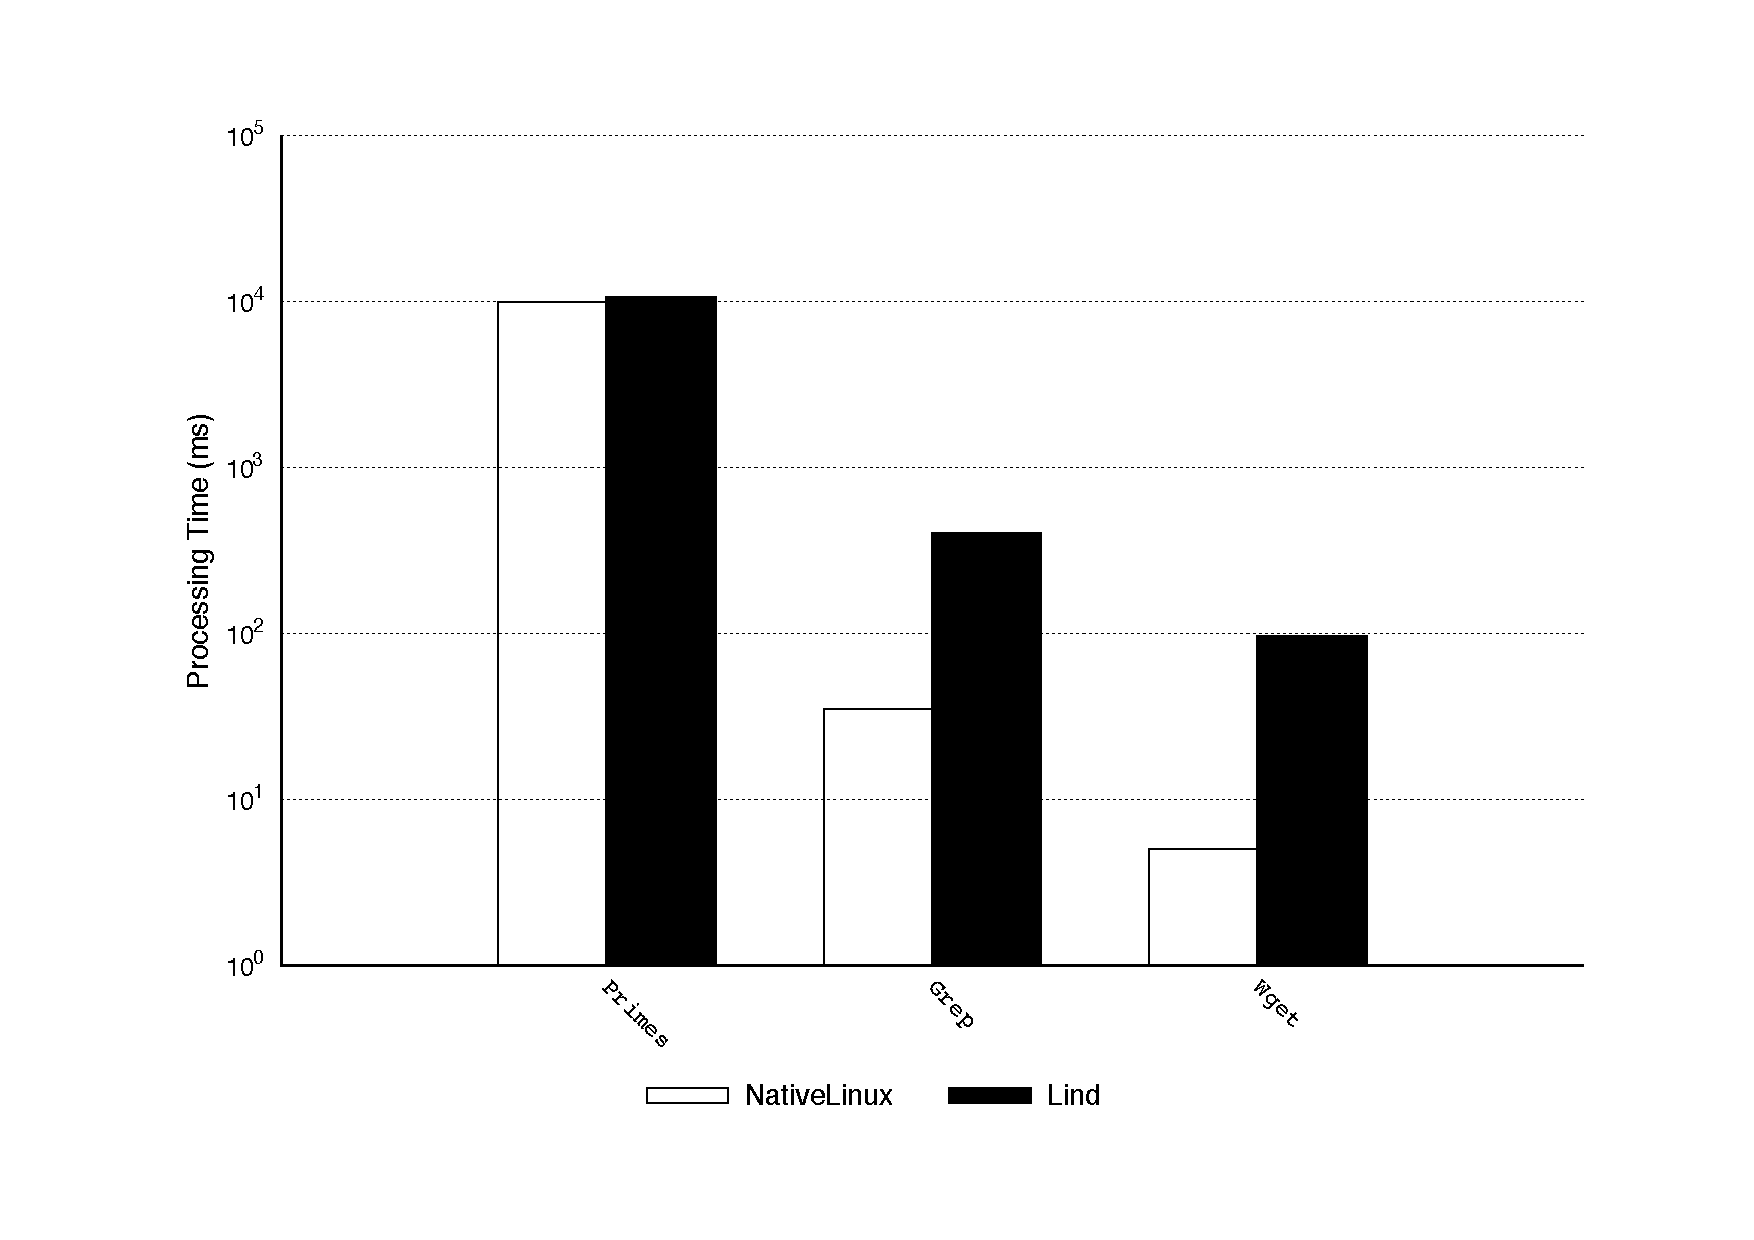
\includegraphics[width=1.0\columnwidth]{diagram/lind_oakland16_performance.pdf}
\caption{Application Runtime Performance: Native Linux vs. Lind}
\label{fig:performance_applications}
\end{figure}

While efficiency was not our main goal, we also evaluated Lind to see
how its performance compared to other systems in a real-world application.
Note that we did not optimize the performance of Lind in any way.

We first compiled and ran three widely used applications:
a primes calculator, GNU \texttt{grep}, and GNU \texttt{wget}. All ran unaltered and
correctly inside Lind. The source code of each of the applications remained
unmodified. To run the applications, it was sufficient to just recompile the
source code using NaCl's compiler and Lind's \texttt{glibc} to call
into SafePOSIX.
Figure \ref{fig:performance_applications} shows the runtime performance
results.
The primes application run in Lind has a 6\% performance overhead compared to
Native Linux. CPU bound applications, like the primes, engender little overhead,
because they run only inside the NaCl computation sandbox. No system calls are required,
and there is no need to go through the safe POSIX interface. The small amount of overhead
is generated by NaCl's instruction alignment at building time. Another reason for the overhead
is that the instructions built by NaCl have a higher rate of cache misses, which can slowdown the
program.
We expect other CPU bound processes to behave similarly.
\texttt{grep} experienced roughly 11x slowdown over Native Linux, while \texttt{wget}
slowdown was roughly 19x. Since they are both I/O heavy applications,
each repeatedly calls into the SafePOSIX code which then reimplements
the call.  The additional computation of SafePOSIX produced the additional
overhead.

Next, we ran the Tor router software in Lind \cappos{what version}. Tor simply
needs to be recompiled to run in Lind.
We used the benchmarks that come with Tor to test its common operations.
A summary of the results is shown in Table \ref{table:performance_tor}. The
benchmarks focus on cryptographic operations,
which are CPU intensive, but also make system calls like \texttt{getpid}, and reads to
\texttt{/dev/urandom}.
The digest operations time the access of a map of message digests.
The AES operations time AES encryptions of several sizes and message
digest creation.
Cell processing executes full packet encryption and decryption. In our
test, Lind slowed down these operations by 2.5x to 5x. We believe these
slowdowns are due to the increased code size produced by NaCl,
\cappos{I'm not sure why this would be.  Does NaCl show this too?}
and the
increased overhead from Lind's safe POSIX system call interface.

As shown above,  Lind incurs some performance overhead in most cases.
It should be noted that, we have not  yet attempted to optimize its performance.
However, since an attack on the kernel has devastating
consequences, %at this initial stage,
a tradeoff between security and performance is well justified.
The fact that Lind is able to run many \cappos{4 applications isn't many...
Do we have Apache numbers or something else to quantify?} legacy applications
suggests that it
is a positive step towards building new secure systems.

\begin{table}
\centering
\scriptsize
\caption{Performance Results on Tor's Built-in Benchmark Program: Native
Linux vs. Lind.}
\begin{tabular}{|r|r|r|r|}
  \hline
  {\bf Benchmark} & {\bf Native Code} & {\bf Lind} & {\bf Impact}  \\
  \hline
  Digest Tests: & & & \\
  Set & 54.80 nsec/element & 176.86 nsec/element & 3.22x \\
  Get & 42.30 nsec/element & 134.38 nsec/element & 3.17x \\
  Add & 11.69 nsec/element & 53.91 nsec/element & 4.61x \\
  IsIn & 8.24 nsec/element & 39.82 nsec/element & 4.83x \\
  \hline
  AES Tests: & & & \\
  1 Byte & 14.83 nsec/B & 36.93 nsec/B & 2.49x \\
  16 Byte & 7.45 nsec/B & 16.95 nsec/B & 2.28x \\
  1024 Byte & 6.91 nsec/B & 15.42 nsec/B & 2.23x \\
  4096 Byte & 6.96 nsec/B & 15.35 nsec/B & 2.21x \\
  8192 Byte & 6.94 nsec/B & 15.47 nsec/B & 2.23x \\
  Cell Sized & 6.81 nsec/B & 14.71 nsec/B & 2.16x \\
  \hline
  Cell Processing: & & & \\
  Inbound & 3378.18 nsec/cell & 8418.03 nsec/cell & 2.49x \\
  (per Byte) & 6.64 nsec/B & 16.54 nsec/B & - \\
  Outbound & 3384.01 nsec/cell & 8127.42 nsec/cell & 2.40x \\
  (per Byte) & 6.65 nsec/B & 15.97 nsec/B & - \\
  \hline
\end{tabular}
\label{table:performance_tor}
\end{table}

\section{Limitations and Future Work}
\label{sec.limitation}

Though Lind shows potential as an effective method for protecting privileged code,
further investigation is required to address issues that were not included in our
initial study.
%We discuss the limitations of Lind in this section.
First, our metric relies on identifying lines of code in the kernel that are
executed when running applications in secure systems.
Our current study only focuses on OS kernel protection, while the area of hypervisor-based
VMs is also very interesting and worth looking into.
It is not clear if
existing hypervisors are small and compact enough to consider all the
identified paths traversing off executing applications as common paths or
whether there is still substantial benefit from our metric.
In %our
future work we will %explore
investigate if the bug metric works well for %operating system virtual machines with a hypervisor.
hypervisor-based VMs.

A second limitation stems from our criteria for determining if a kernel trace is
safe or risky. In our study, the criteria involved checking the trace against a list
 f historical kernel bugs.
 %However, not all bugs can be accurately checked in this manner.
But due to the nature of bugs our proposed metric can not assure if a portion of code
is absolutely a safe or a risky area in kernel.
So we are just trying to reduce the chances of triggering underlying kernel bugs, but can 
not promise to avoid all bugs.
For example, bugs that are caused
by a race condition cannot be identified by directly checking if certain lines of
code have been executed. For complicated bugs that involve defects in the internal
kernel data structures, or require complex triggering conditions across multiple
kernel paths, our metric will not be able to accurately determine whether or not
those bugs have been triggered. In such cases, more complex metrics might be needed
 for detection.

%While Lind executes programs like Apache and Tor, it does not
%support every system call or every possible set of arguments. For example,
%symbolic links are not supported.  While the SafePOSIX implementation could
%be extended to do so, we leave this for future work. Also, as mentioned in
%the previous section,


%There were also some avenues we intentionally excluded in this initial
%study that could form the basis for interesting research projects in the
%future. First, we chose not to explore bugs within the applications
%themselves.
%\cappos{move to motivation / threat model.}

Lind has not been optimized for performance, so the results we present here should be taken as a baseline.
%of what is possible.
We would like to explore what existing OS VM optimizations can be safely applied
and what their impact might be.

We would also like to test our metric in other popular operating systems, such as Windows and Mac OS.
Our experiments were limited to Linux kernel 3.14.1 and some of the typical virtualization systems that existed in Linux.
It would be interesting
%and beneficial to the advance of secure systems
if similar tests could be run in other widely-used operating systems. In particular, it would be interesting to see if
having the host and guest VM run different operating systems would produce different security impacts.

\section{Related Work}
\label{sec.related_work}
This section summarizes other kernel security approaches, such as virtualization
 or other isolation mechanisms
that aim to ensure the safety of privileged code in user space and kernel space.
\lois{Justin and Yanyan: In reviewing this section, consider re-organizing this
literature around how these sources relate to the function of Lind rather than
just techniques used.}

%\lois{Do all of your subtopics fall into this one category? If not,
this introductory sentence should be modified}
ater in another effort, Palix found that \texttt{drivers} still contains the
most faults inthe Linux kernel, in addition to HAL and \texttt{fs}~\cite{palix2011faults}.

\subsection{Early Kernel Metrics}

As mentioned in Section 3, earlier research metrics have suggested a number
of approaches to quantifying risk in the OS kernel.
Palix found that \texttt{drivers} still contains the
most faults inthe Linux kernel, in addition to HAL and \texttt{fs}~\cite{palix2011faults}.
In ~\cite{engler2001bugs} Engler analyzed system code by static analysis
to look for contradictions,such as acquired locks that are
not released.


%Studies have also been conducted based on the number of functions and/or the number of executable lines of code in the function~\cite{Mining-Metrics}.
%\lois[Isn' this a bit repetitious]

Coverage-based fault localization assumes that execution events that occur mostly in failing
test cases, but rarely in passing test cases, are more \textit{suspect}
of being the fault~\cite{jones2002visualization}. Further research in the field lead to measuring the set
difference of the statements covered by passing and failing test scenarios with run-time events~\cite{agrawal1995fault, jones2005empirical}.
Additionally, statistical likelihood testcase with a predicate that evaluates to True
is correlated with failure ~\cite{liblit2005scalable}.\lois{This sentence is somehow incomplete}

%While these metrics can give insight on the possible places where bugs have been located in software systems, they have limitations.
%Firstly, the metrics mentioned above are not specifically designed for studying bugs in OS kernels.
%\cappos{Why does this matter?}

%Therefore, they do not take into account the way system calls are invoked by user applications.
%Moreover, these metrics can not provide information about the accurate location of the bugs within the kernel, which is important to our study.
%\cappos{Are you going to show that this is true?  Can you explain more about why these do not work?}
%\cappos{Do existing metrics work on a LOC level?  }

\subsection{Virtualization}

\textbf{Language-based virtualization.}
Programming languages that provide safety through virtualization such
as Java, JavaScript, Lua~\cite{Lua}, and
Silverlight~\cite{Silverlight} are commonly used in application-level
sandboxing. These safe languages provide virtualized environments to
check the safety of the running code by a monitor process. They
combine untrusted application code with an interpreter and
standard libraries that consolidate routines to perform I/O, network
communication, and other sensitive functions.
%For example, the Java
%Virtual Machine (JVM) \cite{JVM} functions as an application-level
%sandbox to separate untrusted code from the OS in addition to
%performing safety checks for avoiding unauthorized branching in
%memory.
%
There are also sandboxing solutions based on type-safety of programming
languages, i.e. validating through a type-checker \cite{JS-Sandboxing}
or enforcing security policies on an untrusted system through a
reference monitor \cite{JS-Sandboxing1}. %Compared to these approaches,
%the Lind protection model ensures stronger security than just executing the code in a browser's sandbox to isolate untrusted programs.

%Lind enforces strict policies and
%rules to validate all segments of a code before executing it through a
%dual-layer protection.

Though many sandboxes implement the bulk of standard libraries in
memory-safe languages like Java or C\#, flaws in this code can
still pose a threat. In fact, many security critical bugs can be found
in the standard libraries \cite{JavaBugs, Java-Lessons}.
%Researchers have also
%discovered many severe bugs in Java \cite{Java-Lessons}.
Any bug or failure in a programming language virtual
machine is usually fatal. In contrast, Lind with a very small TCB
 (approximately
8,000 LOC) enhances security of privileged code compared to the above. \lois{why?}
%\lois{OK, what does the TCB have to do with these languages?}

%because of the POSIX implementation with Repy to build the sandbox.

\textbf{OS virtualization.}
OS virtualization techniques can be divided into two categories:
%Type-I or Type-II virtualization. Examples of Type-I virtualization
\textit{bare-metal hardware} virtualization, such as VMware ESX Server, Xen,
LXC~\cite{LXC}, BSD�s jail, Solaris zones, and Hyper-V, and
\textit{hosted hypervisor} virtualization such as VMware
Workstation, VMware Server, VirtualPC and the open-source counterpart
VirtualBox.
%
Security by isolation \cite{Qubes}, \cite{Overshadow},
\cite{SecureVM}, \cite{HypSec} is a feature of OS virtualization that
provides safe executing environments through containment for multiple
user-level virtual environments sharing the same hardware. This
approach relies on the VMM to confine untrusted applications within
guest OSs. However, there are limitations due to
the large attack vectors against the hypervisors, including
vulnerabilities of software and configuration risk.
%For example, the
%small code footprint of a hypervisor can become a potential
%vulnerability and lead to serious problems. Maintaining two OSs in
%virtulized environments is among the other issues that add complexity
%\cite{Virt-Issues}. Attackers are able to exploit vulnerabilities to
%escape these systems and access arbitrary code in the underlying host
%systems.
\lois{what is the connection between the above sentences and Lind?}
Lind deals with these concerns by using a much smaller and safer TCB.

\textbf{Library OS.}
Library OSes allow applications to efficiently
obtain the benefits of virtual machines,
including security isolation, host platform compatibility, and
migration. Libra \cite {Libra} is an example of a library OS that allows
applications to customize their OSs within VMs.
This solution is similar to the exokernel approach where a small trusted kernel
 is separated from the untrusted libraries
that function as an abstraction layer between the applications and the underlying hardware.
Libra utilizes a hypervisor instead of the exokernel to deliver efficient
portability and performance. \lois{Ok..so what is the connection}

Drawbridge \cite{Drawbridge-11} is another approach that uses picoprocesses
 (lightweight containers) security monitor (to enforce rules)
and a library OS to present a Windows persona for a wide variety of
Windows applications. Similar to Lind,
it restricts access from usermode to host OS through a number
of operations that pass through the security monitor.
%\lois{How does this fit with Lind?}

%This approach brings many of the benefits of VM based temporal,
%spatial and fault isolation properties to a per-process level.

Bascule \cite{Bascule}, an architecture for library OS extensions
based on Drawbridge, allows application behavior to be customized by
extensions loaded at runtime.
Graphene \cite{Graphene-14} is a recent library OS system that
seamlessly and efficiently executes both single and
multi-process applications, with low memory and performance overheads.
%It broadens the library OS paradigm to support secure, multi-process
%APIs, such as copy-on-write fork, signals, and System V IPC.
Haven \cite{Haven} uses a library OS to implement
shielded execution of unmodified server applications
in an untrusted cloud host.
%Haven leverages the hardware protection of
%Intel SGX to defend against
%privileged code and physical attacks, such as memory probes, but also
%addresses the dual challenges of
%executing unmodified legacy binaries and protecting them from a
%malicious host.
Its library OS technique is similar to Lind but differs in
that existing library OS systems rely heavily on
the underlying kernels to perform system functions. In contrast, Lind only
relies on a very limited set of system functions,
and reconstructs most OS functions with its own safe Repy code.

\subsection{System Call Interposition}

System call interposition (SCI) provides
%offers a number of properties that make it attractive to run applications
secure execution of applications by exposing a minimal kernel surface.
This approach usually ensures the userspace policies through a monitor process that
interacts with the system call execution engine.
%for building sandboxes, though it can be error prone
\cite{SCI-04}.
%Approaches for delegation and filtering have been extensively studied. For example,
%along with their respective tradeoffs between security and
%performance.
Janus (J2) \cite{Janus0:96, Janus:99} is an SCI solution for confining untrusted applications that includes system call filtering
and sandboxing mechanisms.Garfinkel et al. in another effort, introduces Ostia \cite{SCI-04}, where system calls are delegated to
agents that enforce the policies. Ostia resolves the tight dependencies with the underlying OS through process emulation and
the agents model at the userspace. Other issues in utilizing SCI solutions include the difficulty of appropriately replicating OS semantics,
multi-threaded applications that cause race conditions, or indirect paths to resources that are often overlooked.
In addition, system calls that are denied can cause inconsistencies that are discussed in \cite{Problems-SCI}.

Recently, Wang et al. \cite{Jitk} discuss the issues of traditional SCI systems
in the context of in-kernel interpreters such as Seccomp, which is used by several
security critical applications, including Chrome, OpenSSH and Tor.
The authors propose Jitk architecture to avoid the weaknesses in traditional
kernelspace system call interceptors that arise from the unforeseen bugs within
the interceptors. Jitk provides a formal verification tool that ensure the
correct translation of the userspace submitted code, e.g. the  the BSD packet filter and INET-DIAG.

%The kernel module enforces policy, denies direct access to restricted
%resources, and delegates certain calls to an emulation library.
%which sends transformed system calls to the agents.
%The agent reads the policy file and handles the delegation of calls.


%Nevertheless, this technique is very useful and has inspired many new techniques, such as library OSes.
%The concepts behind system call interposition have evolved into other modern techniques and has benefited many security systems, including Lind.

The SCI approach is very similar to the Lind isolation mechanism but a key difference is the actual execution
of a system call through the Lind's reimplementation to ensure safe POSIX API for the userspace applications.

\subsection{Software Fault Isolation}
Software fault isolation (SFI) is an alternative to hardware memory
protection when running two applications in one address space. SFI provides sandboxing in which native
instructions can only be executed if they do not violate the sandbox's
constraints \cite{SFI:93}, and security policies are enforced through machine-level
code analysis. In this approach, memory
writes are protected and code jumps cannot access predefined memory of
other programs to execute their codes.

The preliminary design of SFI was build on RISC
architectures. The authors of PittSFIeld \cite{PittSFIeld} optimized and
extended the original SFI to support CISC architectures.
%For this purpose, the source instructions are padded with no-ops to fit, i.e.
%in the 16-byte x86 byte chunk alignment, where a call instruction is
%appended. A sequence of instructions form a instruction streams that
%ensures execution order of the sequence. The final code before
%execution will be checked by a verifier component to ensure safety.
%
SFI has been also used in MisFIT \cite{MISFit} to ensure kernel
module integrity for x86. The authors emphasized the
extendability of object-oriented programming languages to eliminate
the need for remote calls to achieve high throughput.
%
Nooks \cite{Nooks:03} is another SFI-based solution that provides
a protected environment for running device drivers by isolating kernel
modules. Nooks' runtime environment is located within the
kernel and it includes the majority of drivers that needs to be protected
from each other.
These SFI containers embody the extensions to demonstrate the integrity
validation check in conjunction with the host environment resources.
%i.e. network nook and video nook are two protection
%domains without the possibility for memory writes outside their
%protection domain. The Nook layer function as a reference monitor
%between device devices and physical hardware by forwarding interrupts
%Nooks also wrap calls from the operating system kernel into device
%drivers and from device drivers into the kernel, allowing the
%operating system to track resource usage and verify data that is
%passed into and out of the kernel. Object tracking to allow OS for
%resource consumption is another feature of wrappers in Nooks.

%To enforce the safety constraints, programs demand a specific compiler
%in advance to validate and load the programs. For example, in
Another SFI system called Byte
Granularity Isolation (BGI) \cite{Castro-BGI} was introduced as a runtime tool to isolate drivers in
separate protection SFI domains, while sharing the same address space
between different domains.
%BGI mainly ensures write-integrity,
%control-flow integrity and type safety for kernel objects. For this
%purpose, a BGI compiler is required to transform the unmodified driver
%source code to instrumented driver. The instrumented driver will be
%linked to the BGI interposition libraries that enforce the protection
%constraints to produce the BGI drivers. The protection constraints
%that are enforced by the interposition library are implemented in
%access control lists (ACL). The ACLs contain policies for each byte of
%virtual memory and domain permissions.
A major issue of BGI is that it
does not solve the vulnerabilities at kernel-levels.

Recently, Google provided Native Client (NaCl) \cite{NaCl-09} for
Chrome browser to allow native executable code to be run directly in a
browser using the PittSFIeld semantics. NaCl prevents suspicious code
from memory corruption or direct access to the underlying system
resources. For this purpose NaCl loads untrusted modules from the
trusted modules into two different address spaces, where in most SFI
approaches both untrusted and trusted codes are loaded into a common
address space.

%Mao et al. \cite{LXFI} study the shortcomings of XFI \cite{XFI} and
%BGI \cite{Castro-BGI} kernel module isolation mechanisms that separate
%kernel modules from the core kernel. Integrity of API calls was one of
%the challenging issues in existing solutions. For example in XFI there
%were no argument validation. LXFI solution was proposed as an
%extension of existing SFI solutions with language annotation. LXFI
%added argument integrity in XFI and call back integrity in BGI in
%addition to enabling programmers for specifying principals for access
%permissions within a module.
%
%In another effort \cite{PSFI}, Kroll et al. discuss the issues of
%machine-level SFI that causes portability limitations across different
%hardware architectures. The authors propose portable SFI through a
%higher level of abstraction at the compiler layer. To this end,
%programs are rewritten by an intermediate-level language compiler to
%comply with policies.
\section{Conclusion}
\label{sec.conclusion}

%The idea of isolating untrusted user applications from the underlying privileged code
%to avoid its exploitation by bugs has been realized in different implementations,
%but there is no standard method for creating this isolation.
%In addition, experience suggests that isolation by itself does not guarantee the security of a system.
%
In this paper, we proposed a new metric based on quantitative measures derived from
the execution of kernel code when running user applications.
We verified the hypothesis that commonly used kernel paths contain fewer bugs.
%Using our metric, we generated findings that suggest the hypothesis is reasonable,
% and it become the key principle behind a new design for building secure systems,
Our metric was used to implement a new virtualized security system called Lind. Designed with a minimized
TCB and interacting with the kernel in only commonly used paths, Lind addresses the need to 
support risky system calls by securely reconstructing complex, yet essential OS functionality inside a sandbox.
%
Evaluation results have shown that Lind is the least likely to trigger zero-day Linux kernel bugs,
when compared to seven other virtualization systems, such as VirtualBox, VMWare Workstation, Docker, LXC, 
QEMU, KVM and Graphene.
%This suggests that systems using our design are likely to be more secure.

All of the data and source code for this paper is available at our Lind website~\cite{Lind}. 
For further information and questions, please contact the authors. 
%For access to the kernel exploit code created in this study, please contact the
%authors.


%%%%%%%%%%%%%%%%%%%%%%%%%%%%%%%%%%%%%%%%%%%%%%%%%%%%%%%%%%%%%%%%%%%%%%
%  Bibliography
%%%%%%%%%%%%%%%%%%%%%%%%%%%%%%%%%%%%%%%%%%%%%%%%%%%%%%%%%%%%%%%%%%%%%%


{
\footnotesize
\bibliographystyle{acm}
\bibliography{paper}
}


%\theendnotes

%%%%%%%%%%%%%%%%%%%%%%%%%%%%%%%%%%%%%%%%%%%%%%%%%%%%%%%%%%%%%%%%%%%%%%
%  The End
%%%%%%%%%%%%%%%%%%%%%%%%%%%%%%%%%%%%%%%%%%%%%%%%%%%%%%%%%%%%%%%%%%%%%%


\end{document}
